%!TEX root = ../main.tex
\chapter{Commissioning of the AHCAL technological prototype}
\label{chap:Commissioning}

Before any beam measurement, all the electronics of the detector has to be characterized. Before the full assembly, each individual ASIC must be tested in order to reject the ones that present bad channels or any other defects. After the assembly, each HBU needs to be characterized. This includes the measurement of the SiPM-tile gain, the trigger threshold and electronic noise. In this chapter, the testing of the ASICs and the commissioning procedure of the AHCAL will be presented.

\section{Testing of individual SPIROC2B chips}

The testing of individual chips prior to the soldering to the HBU board is necessary. This avoids broken chips to be installed and reduces the number of dead channels. In the past, OMEGA was testing the functioning of the SPIROC ASICs and classify it into 3 grades: A, B and C grades. Only A-grades ASICs were used. The testing is done manually for each chip as no fully automatic testing setup was available at the time of testing. This reduces the number of cross-checks done on the chips due to time constraints. The SPIROC2B chip (see section \ref{sec:SPIROC2B}) can be tested standalone on a custom made PCB board. The SPIROC2B chip is installed in a special socket and is read-out by an ALTERA \acrshort{fpga}. The board is operated by a Labview software made by the OMEGA group \cite{OmegaWeb}.

\begin{figure}[htbp!]
  \centering
  \begin{subfigure}[t]{0.49\textwidth}
    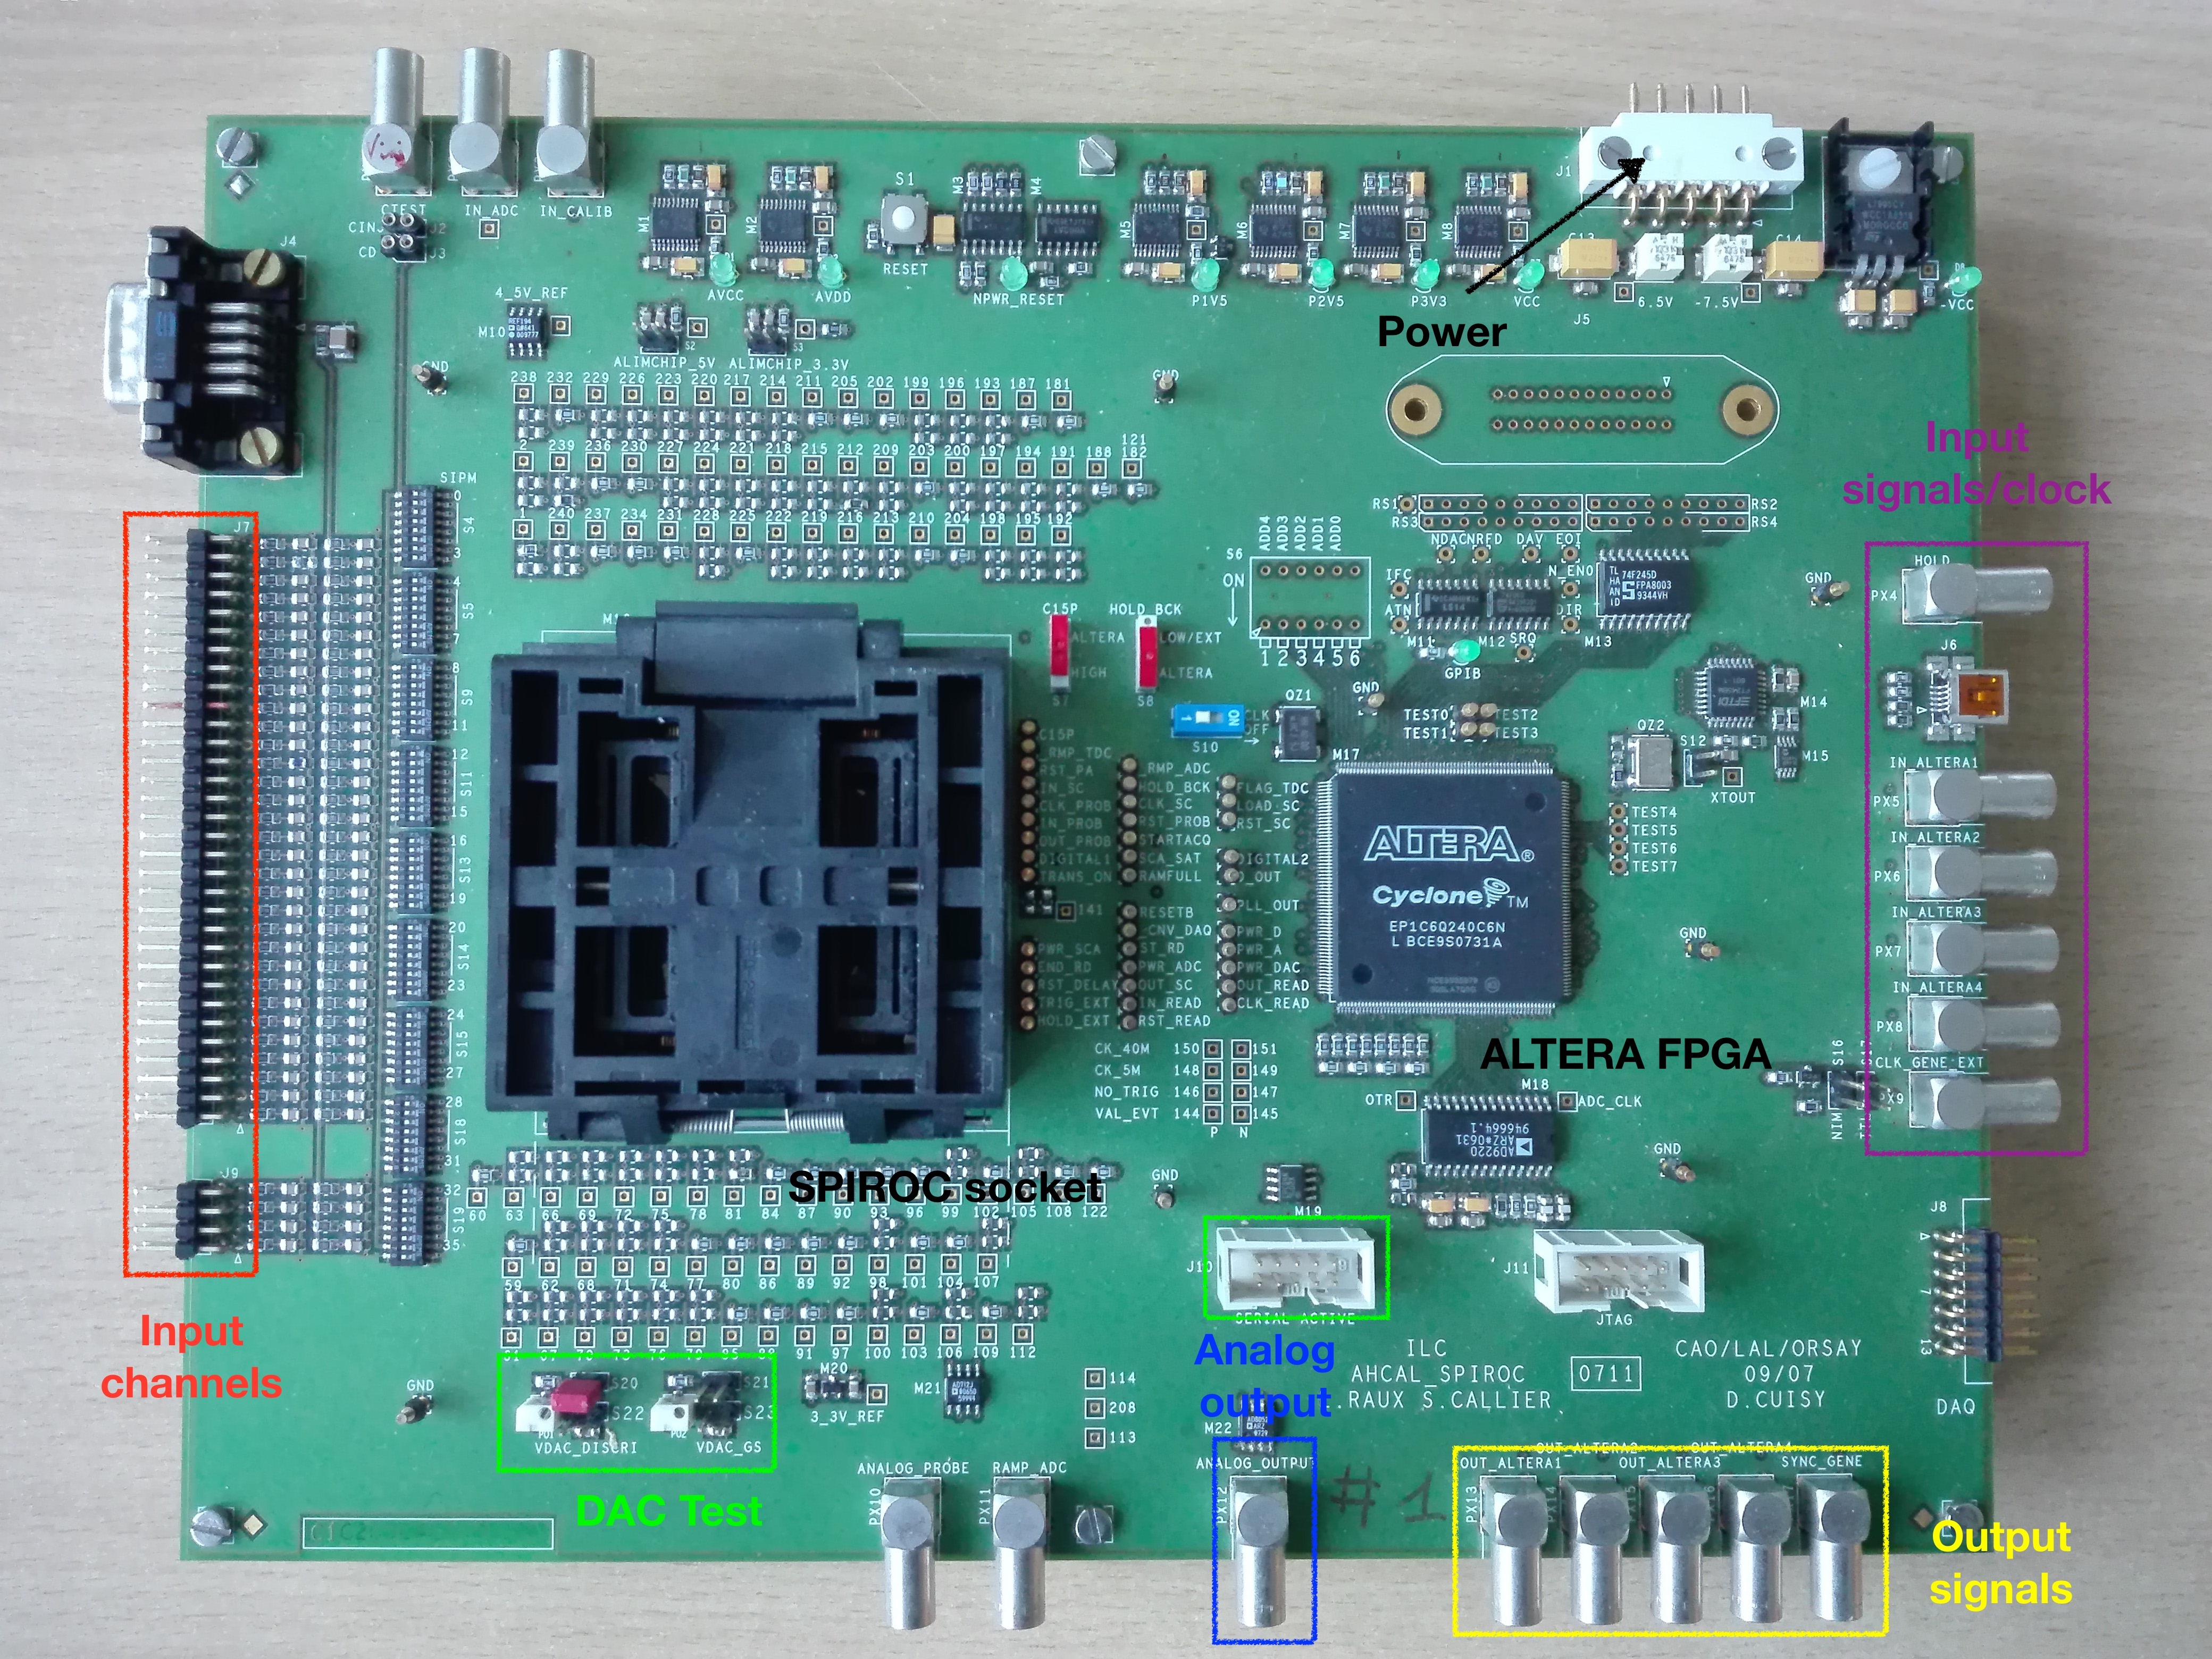
\includegraphics[width=1.\linewidth]{chap4/fig_Commi/TestBoard.jpg}
    \caption{} \label{fig:Testboard_SP2B}
  \end{subfigure}
  \hfill
  \begin{subfigure}[t]{0.49\textwidth}
    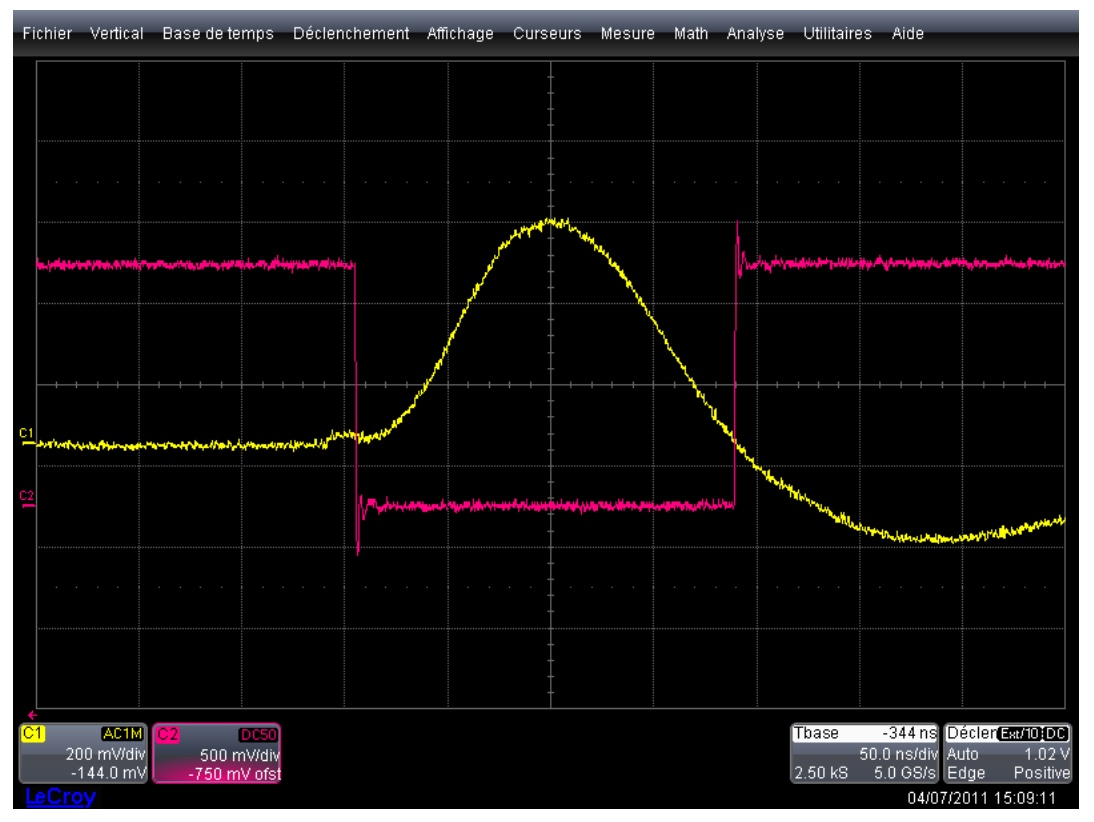
\includegraphics[width=1.\linewidth]{chap4/fig_Commi/AnalogSignalSP2B.jpeg}
    \caption{} \label{fig:AnalogSignal_SP2B}
  \end{subfigure}
  \caption{\subref{fig:Testboard_SP2B}) Testboard used to test the SPIROC2B chip standalone. The red square represents the 36 input channels of the SPIROC ASIC, the purple square represents the input signals for the ALTERA such as clocks. In yellow and blue squares represent the output signals, analog and digital, of the SPIROC. The green square, above the blue and yellow one, represents the input and output DACs that can be measured automatically via a Keithley multimeter with the Labview software. \subref{fig:AnalogSignal_SP2B}) Example of an analog signal outputted by the slow shaper of the SPIROC2B. The signal is represented in yellow. The trigger is represented in red.}
\end{figure}

The board as shown in figure \ref{fig:Testboard_SP2B} contains all the debugging features needed to check the functioning of the chip. The red square represents the input signal for the 36 channels. Generally, a SiPM like-pulse with a fast rising edge (around 1 ns) and a slower falling edge (around 20 ns) is injected into one channel of the chip.

In the blue and yellow square are the output signals. This enables to check via an oscilloscope the output analog signal after the slow shaper, but can only be checked in external trigger mode. This is shown in figure \ref{fig:AnalogSignal_SP2B}, the signal from the SiPM is integrated over a long period (typically 100-200 ns) and it enables to easily sample the signal at the maximum.

In the purple square are the input signals for the FPGA such as the slow clock and external trigger signals. And finally, the green square (above the blue and yellow squares) represents the \textit{trigger threshold} and the channel-wise voltage adjustment \textit{Digital to Analog Converters} (DAC) that can be tested manually or automatically by connecting a Keithley multimeter a serial port on the board.

In this manual procedure, the vital parts of the chips are tested. This includes to check that all channels are working correctly, that the chip works in both external and auto-trigger modes, that all both the trigger threshold and the voltage adjustment DACs are working and that the digital part converts and sends the data out of the chip. For the testbeam in July 2015, around 60 chips have been tested manually for the layers 12, 13 and 14. The mean time for testing a chip is around ten minutes.

\subsection{DAC Testing}

As the testing procedure is done manually, only the most critical components of the chip are tested. One of this component is called the DAC. Two DACs are present in the SPIROC2b. One is regulating the channel-wise voltage applied to the SiPM (8-bit input DAC) and another is controlling the trigger threshold discriminator (10-bit output DAC) which is common to the 36 channels. In the following, the DAC regulating the voltage channel-wise is referred as the input DAC and the DAC controlling the trigger threshold is referred as the output DAC.

The measurement procedure is done in two parts for the input DAC. First, a simple check is done by measuring the voltage of the channel at a DAC value of 0. If one of the channels presents an unstable voltage, it indicates likely that the input DAC for this channel is broken thus the chip is discarded. If a chip passes the simple check, then the input DAC curve for all channels is measured with a Keithley multimeter connected to a serial port on the board. The measurement is done automatically with the Labview software. The time required is around 1-2 minutes per chip.

The output of the measurement is a list containing the DAC value (from 0 to 128) and the associated voltage. The reconstructed input DAC curve is shown in figure \ref{fig:IDAC}. One can notice that the spread channel-to-channel for the input DAC increases with the value. The spread is around 10 mV at a value of 0 and goes up to 200 mV at a value of 128. For older generation SiPMs, fine voltage adjustment was needed to reduce the spread in gain due to a wide spread in breakdown voltages \cite{Hartbrich2012}. For newer generation SiPMs and new produced modules, the spread in breakdown voltage is very small (less than 100 mV) and, therefore no voltage adjustment is needed anymore. For the testbeam in this thesis, a DAC value of 0 was chosen where the spread is minimal.

\begin{figure}[htbp!]
  \centering
  \begin{subfigure}[t]{0.49\textwidth}
    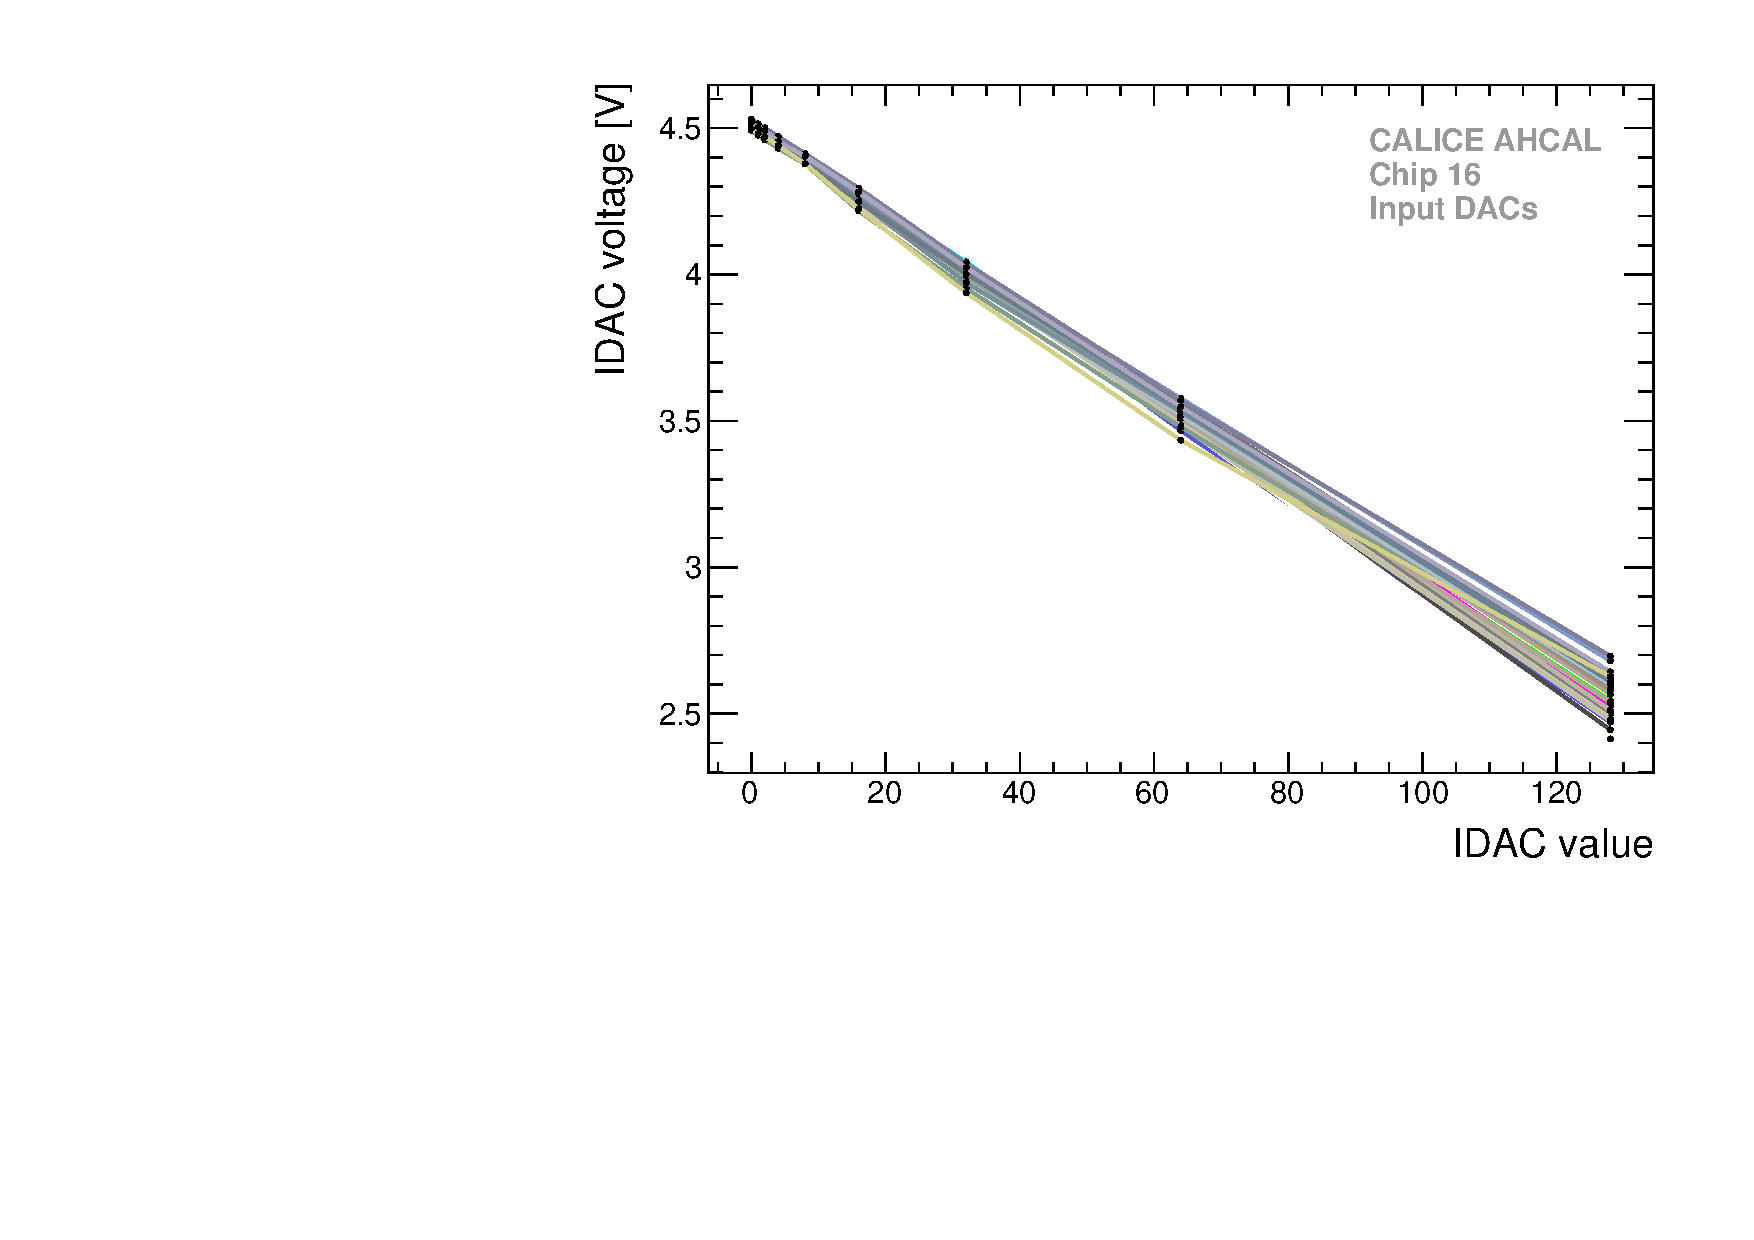
\includegraphics[width=1.\linewidth]{../Thesis_Plots/Commissioning/Plots/IDACs_Chip16.pdf}
    \caption{} \label{fig:IDAC}
  \end{subfigure}
  \hfill
  \begin{subfigure}[t]{0.49\textwidth}
    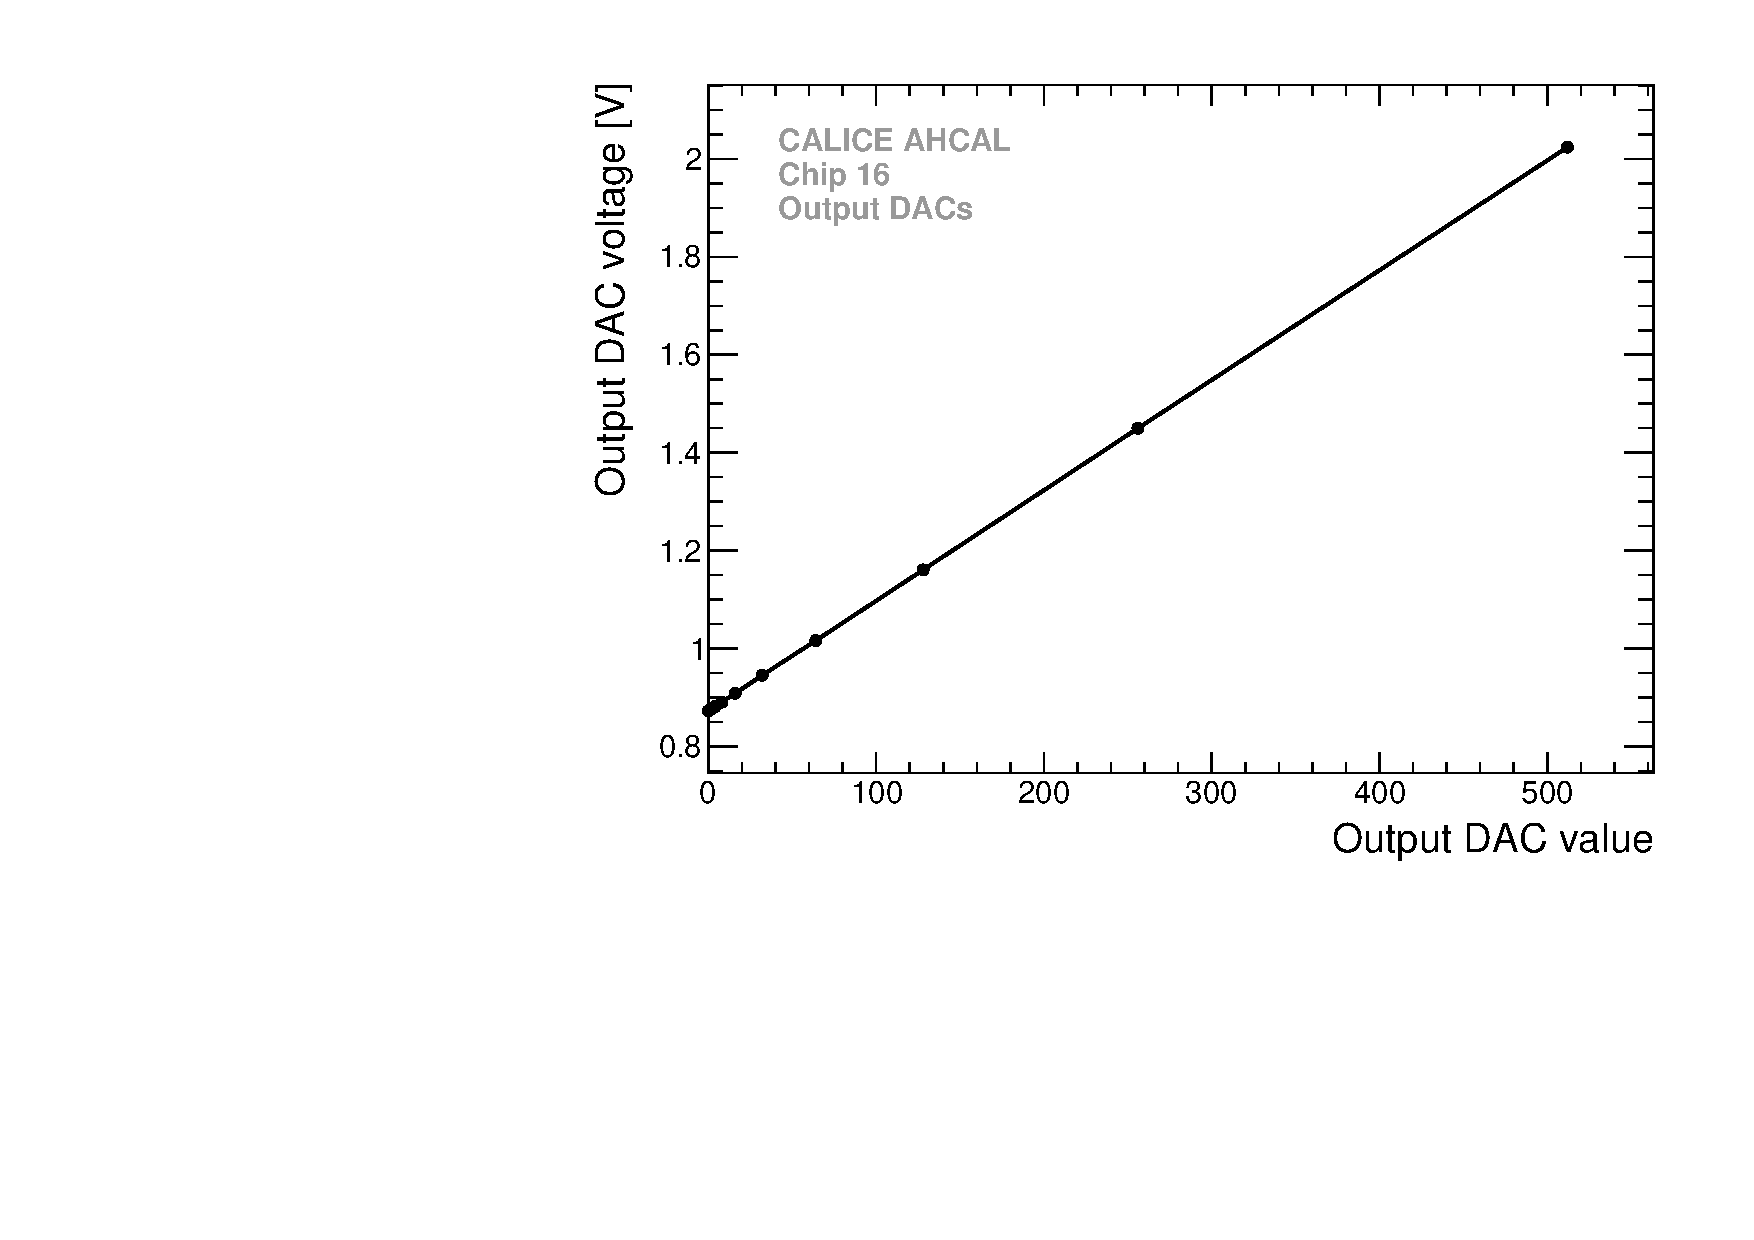
\includegraphics[width=1.\linewidth]{../Thesis_Plots/Commissioning/Plots/OutDACs_Chip16.pdf}
    \caption{} \label{fig:OutDAC}
  \end{subfigure}
  \caption{\subref{fig:IDAC}) Reconstructed input DAC curves of the 36 channels for the Chip 16 of the tested batch. \subref{fig:OutDAC}) Reconstructed output DAC curve for same tested chip.}
\end{figure}

For the output DAC, a Keithley multimeter is connected to a second serial port on the board and measures the output DAC automatically with the Labview. The output of the measurement is a list containing the output DAC value from 0 to 512 and the associated voltage. The reconstructed curve is shown in figure \ref{fig:OutDAC}. The output DAC for this chip has a linear behavior as expected. If any other behavior was observed, the chip was discarded.

\begin{center}
  \rule{0.5\textwidth}{.4pt}
\end{center}

Around 60 chips were tested with a yield of 84\%. There is no obvious common cause for failure (digital part not working, no response to slow control programming, broken input DAC...). The time to test a chip manually is around 10 minutes. A new testing board has been designed by DESY and the University of Wuppertal in order to automatize the testing procedure of individual chips on \acrshort{bga} packaging \cite{AHCALMain2016_Amine} and to reduce the time needed for the testing procedure. This new board has been commissioned in July 2017 and it is being used currently for the next generation AHCAL prototype to test around 650 chips.

\section{HBU Commissioning procedure}

The commissioning procedure of the detector was done in July/August 2014 for a testbeam that was planned in October/November 2014 at the CERN PS facility. Mainly, the same boards were used during the testbeams in 2015. A picture of the setup used in this thesis is shown in figure \ref{fig:Det_layout}. Before the assembly of the detector into the absorber stack, each individual HBU needs to be tested. This test is done in order to characterize the full board. The procedure is explained in detail in \cite{Hartbrich2012} and was done with these steps:

\begin{itemize}
  \item The setup the Power Board voltage to deliver the high voltage to the SIPM and the setup the input DAC value.
  \item A first characterization of the board by measuring the SiPM gain at nominal settings.
  \item An iterative adjustment of the pre-amplifier gain to reach the targeted SiPM gain.
  \item A threshold scan measurement.
  \item A noise measurement.
\end{itemize}

The following subsections will describe each point in more detail. The layer 3 and layers 12 to 14 (13 HBUs) were fully commissioned. The layers 4 to 11 (11 HBUs) have already been calibrated in the past and they used the same pre-configured settings. Only a cross-check was performed for these layers. The layers 1 and 2, the ECAL boards (EBUs), were commissioned separately due to high noise and very low gain.

\subsection{Setting the High Voltage}

\begin{table}[htb!]
  \centering
  \caption{List of the different SiPMs used in the CALICE AHCAL in July 2015.}
  \label{table:sipm_list}
  \resizebox{\textwidth}{!}{%
  \begin{tabular}{@{}cccccccc@{}}
    \toprule
    Layer & Producer & Model & Area (mm$^2$) & Pitch ($\mu$m) & WLS Fibre & Read-out type & $N_{px}$ [$10^3$]\\
    \midrule
    1 & Hamamatsu & S12571\_010P & $1\times1$ & 10 & no & Bottom & 10\\
    2 & Hamamatsu & S10362-11-025O & $1\times1$ & 25 & no & Side & 1.6\\
    3 & Hamamatsu & S12571-025P & $1\times1$ & 25 & no & SMD & 1.6\\
    4-5 & Ketek & N/A & $2.25\times2.25$ & 18 & no & Side & 12\\
    6-10 & CPTA & CPTA & $1.28\times1.28$ & 40 & yes & Side & 0.8\\
    11-12 & Ketek (UHH) & PM1125NS-SB0 & $1.2\times1.2$ & 25 & no & Side & 2.3\\
    13-14 & SenSL & MicroFB-10020-SMT & $1\times1$ & 20 & no & Side & 1.3\\
    \bottomrule
  \end{tabular}
  }
\end{table}

An AHCAL board (HBU) has 144 channels, each equipped with a plastic tile-SiPM. To achieve a certain light yield, i.e the number of fired pixels per MIP, the SiPM must be operated above a specific voltage called the breakdown voltage $V_{Br}$ (see section \ref{sec:SiPM}). This voltage has been measured for a couple of SiPMs. For newer generation SiPMs, it is given by the manufacturer where batches of SiPMs are placed in bags with a certain $V_{Br}$ and the lower/upper limits are indicated. The table \ref{table:sipm_list} shows the SiPMs used during the testbeam at CERN in July 2015. The variation of the breakdown voltage is in the order of hundreds of millivolts between SiPMs of the same type.

The SiPMs are operated between 2.5 to 5V over the breakdown voltage depending on the type. The high voltage that is set on the power board $V_{PB}$ is determined by the distribution of the SiPM bias voltages of each HBU taking into account a safe margin for the voltage adjustment with the input DAC. Then, the input DAC for each channel is calculated to have the targeted SiPM bias voltage. This made the procedure very laborious and time-taking \cite{Hartbrich2012}.

As the quality of SiPMs has increased drastically in the last few years, the need for individual channel-wise voltage is reduced. This simplifies the procedure to $V_{PB} [V] = V_{Br} + V_{overvoltage} - V_{IDAC}$ where $V_{IDAC}$ is fixed and common to all channels. The table \ref{table:Voltage_SiPM} sums up the voltages applied.

\begin{table}[htb!]
  \centering
  \caption{List of breakdown and operating voltages applied to each SiPM types. $V_{op}$ represents $V_{Br} + V_{overvoltage}$.}
  \label{table:Voltage_SiPM}
  \begin{tabular}{@{}lccc@{}}
    \toprule
    SiPM type \# & $V_{Br}$ & $V_{op}$ & $V_{PB}$\\
    \midrule
    Hamamatsu (S12571\_010P - S10362-11-025O) & $\sim$ 65 V & $\sim$ 70 V & $\sim$ 75.8 V\\
    Hamamatsu (S12571-025P) & $\sim$ 65 V & $\sim$ 67 V & $\sim$ 70.66 V\\
    CPTA (layers 6-10) & $\sim$ 35-45 V & $\sim$ 37-50 V & $\sim$ 40.1 - 51.7 V\\
    Ketek (layers 4-5) & $\sim$ 28 V & $\sim$ 32 V & $\sim$ 36.95 - 37.02 V\\
    UHH Ketek (layers 11-12) & $\sim$ 27 V & $\sim$ 29.55 - 30.05 V & $\sim$ 32.98 - 34.49 V\\
    SenSL (layers 13-14) & $\sim$ 25 V & $\sim$ 27.391 - 27.392 V & $\sim$ 32.10 - 32.11 V\\
    \bottomrule
  \end{tabular}
\end{table}

\subsection{First characterization of the gain}
\label{subsec:GainCharac}

In this section, the SiPM gain is related to the ADC value between the two first peaks of a single pixel spectrum where individual pixels, in a relatively small number ($\sim$10-15 pixels), are fired by an integrated LED system. This value is proportional to the high voltage applied to the SiPM and can be also modified by adjusting a feedback capacitor of the SPIROC2B high gain pre-amplifier.

Before starting the gain measurement procedure, a holdscan needs to be performed. The hold time is the time delay between the trigger and the sampling of the signal after the slow shaper. This time needs to be chosen in order to sample the maximum of the signal. The procedure aims to reconstruct the signal shape after the slow shaper by injecting a fixed amplitude signal using the integrated LED system to all the channels while repeating this for several hold time values from 0 to 60 ns.

Only channels where the integral of the curve is above 6000 are chosen. This is done to reject channels presenting a curve too flat that would make the determination of the hold time difficult. The results for a typical chip are shown in figure \ref{fig:Holdscan}. The hold time value is chosen by eye where the maximum of the signal is.

\begin{figure}[htbp!]
  \centering
  \begin{subfigure}[t]{0.49\textwidth}
    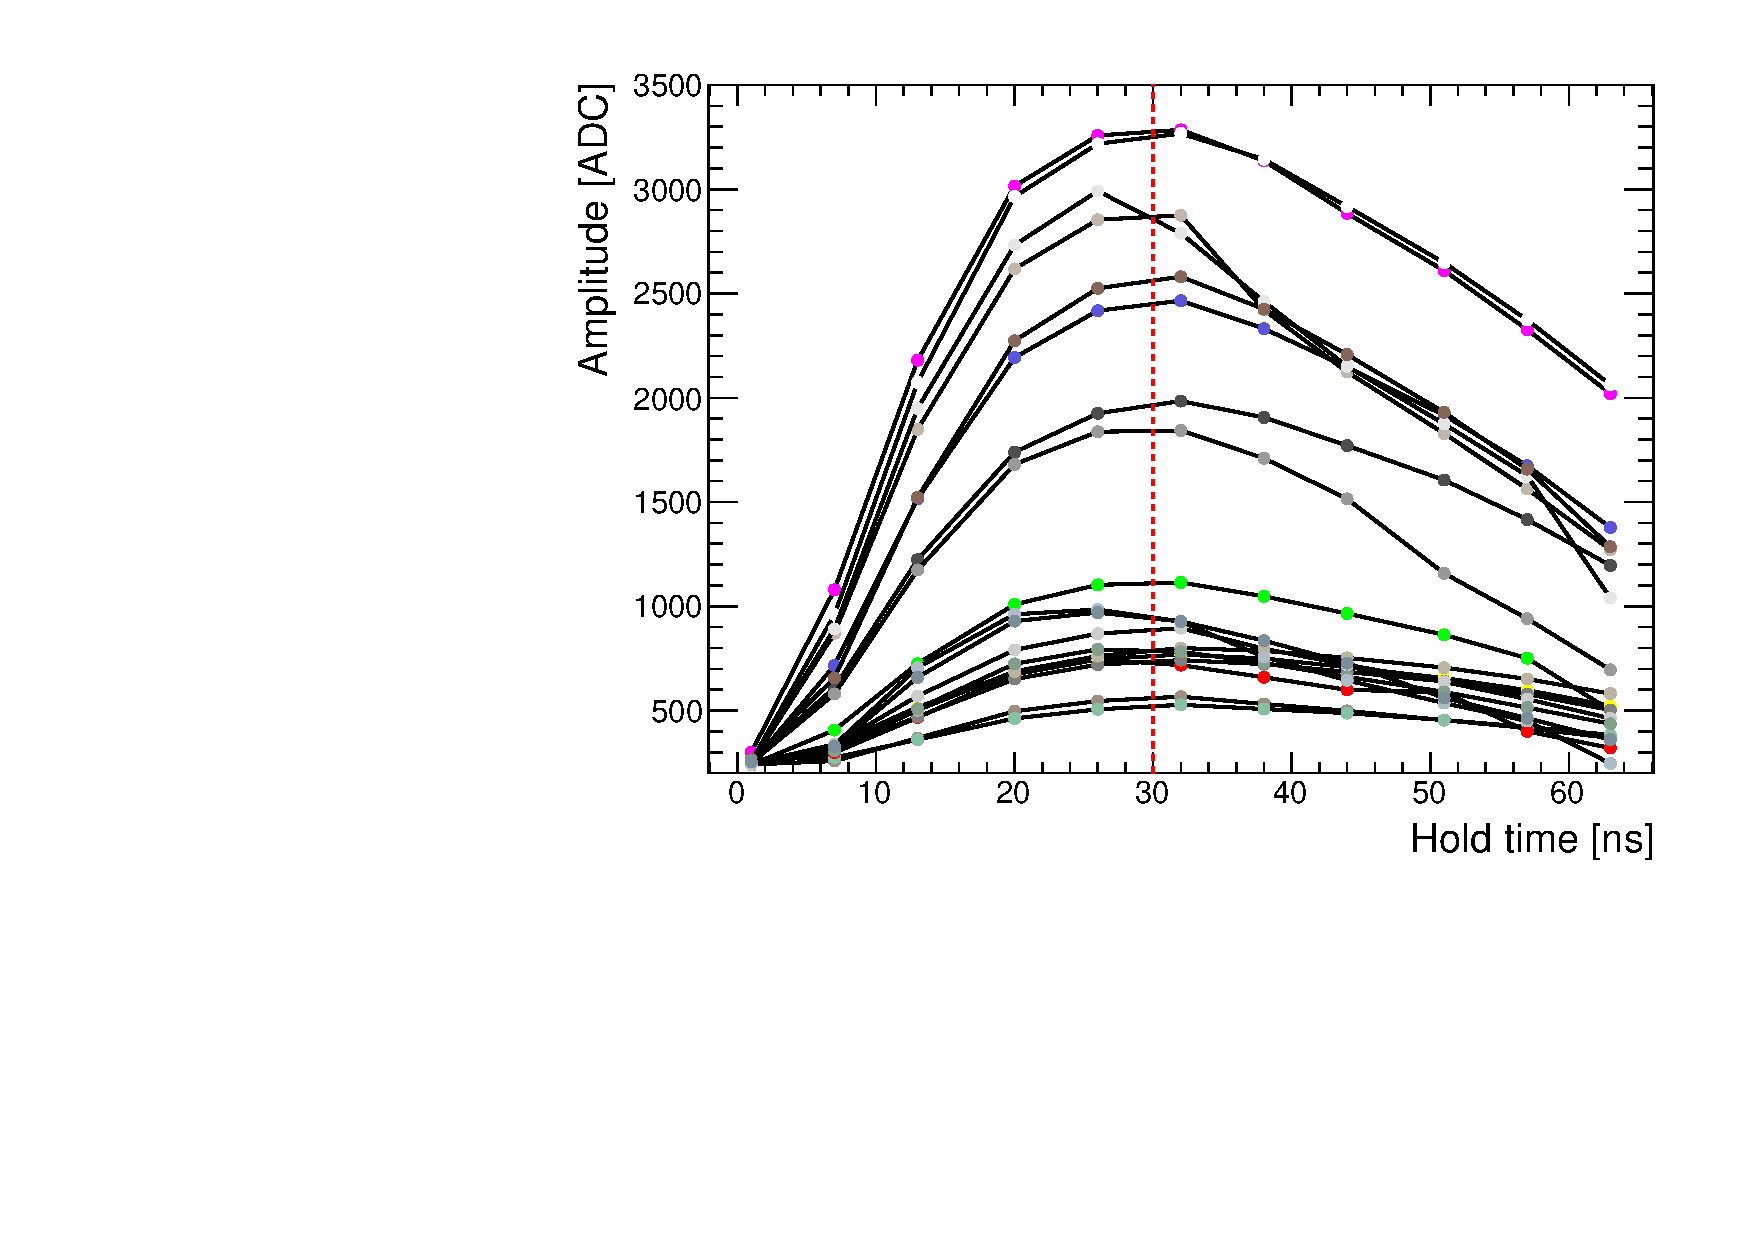
\includegraphics[width=1.\linewidth]{../Thesis_Plots/Commissioning/Plots/Holdscan_HBU2_15.pdf}
    \caption{Holdscan} \label{fig:Holdscan}
  \end{subfigure}
  \hfill
  \begin{subfigure}[t]{0.49\textwidth}
    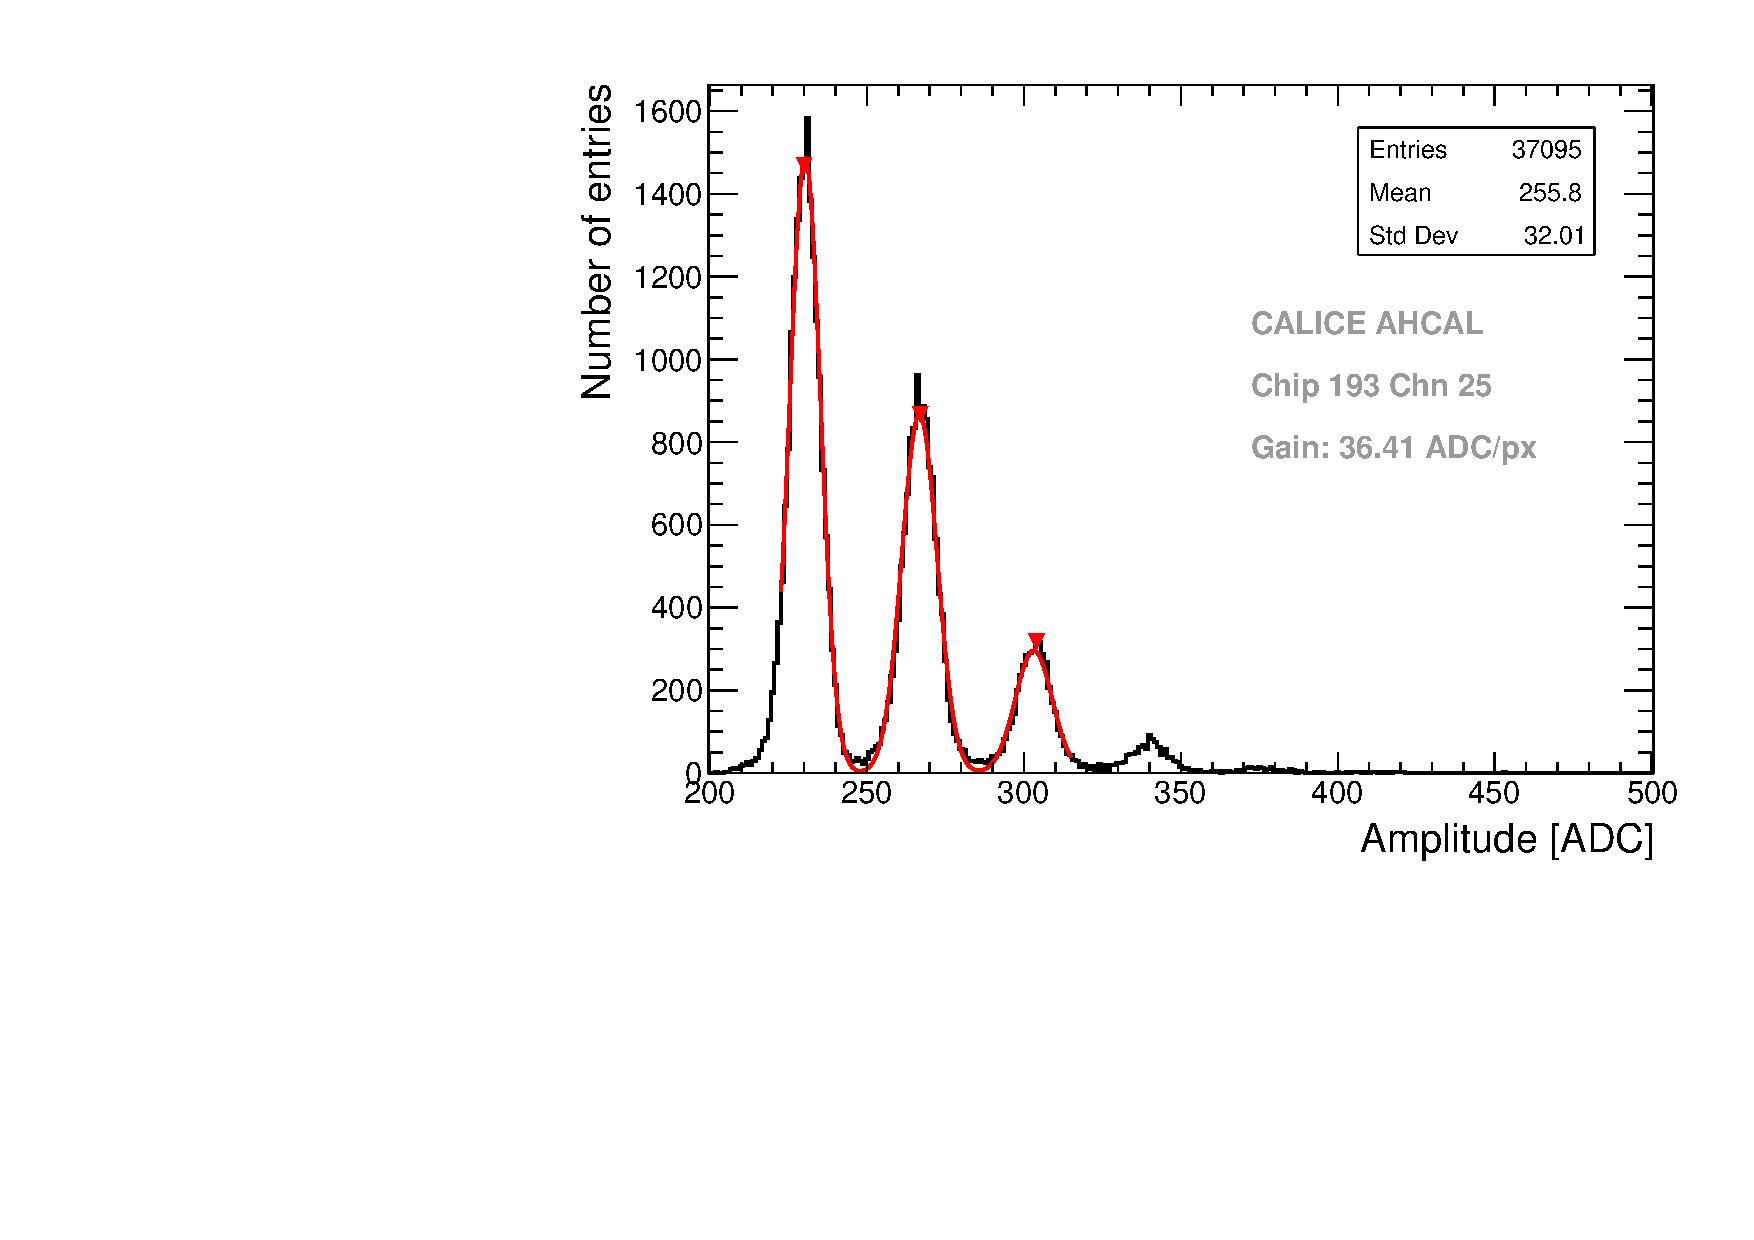
\includegraphics[width=1.\linewidth]{../Thesis_Plots/Commissioning/Plots/Gain100fF_MainzHBU4.pdf}
    \caption{Gain measured at 100 fF} \label{fig:Gain100fF}
  \end{subfigure}
  \caption{\subref{fig:Holdscan}) Reconstructed signal shape for several channels of Chip 174 on HBU\_{}2\_{}15 (layer 11). Only channels where the integral of the holdscan curve is over 6000 are shown. The dotted red line represent the Hold time chosen for this board. \subref{fig:Gain100fF}) Single pixel spectrum of a single channel. The fit is done by a Multi-Gaussian where the distance between the 1$^{st}$ and 2$^{nd}$ peaks is the fitted SiPM gain.}
\end{figure}

After this, a first characterization of the gain can be done at nominal settings using a pre-amplifier value of 100 fF. For this, all channels are illuminated by the integrated LED system with a certain range of LED voltage in steps of 100 mV in order to characterize all channels due to variations in response due to LED light, tiles, SiPM. For layers 4 to 11, a range of 10-15 voltages are needed. Due to improvements in the integrated LED calibration system design, SiPM quality and tile quality, a much smaller range can be used (3-5 voltages) for the layers 3 and 12 to 14. A typical example of a single pixel spectrum at 100 fF can be seen in figure \ref{fig:Gain100fF}.

\subsection{Adjustment of the ADC dynamic range}

The goal of this procedure is to fit the dynamic range of the SPIROC2B in ADC to the number of pixels on the SiPM to avoid any ADC saturation before SiPM saturation. ADC saturation would mean that information is lost and as well that the full range of pixels on the SiPM would be not used. This calculation is still approximate due to several unknown variables such as the number of effective pixels of a SiPM and the calibration factor between the high gain and the low gain for each channel called the intercalibration factor but this procedure gives a good order of magnitude for the target gain.

The targeted gain is calculated by:
\begin{equation}
  G_{target} [ADC] = \frac{ADC_{max}}{N_{px} [px]}
\end{equation}
where $G_{target}$ is the value targeted for gain, $ADC_{max}$ is the maximum ADC range and $N_{px}$ the number of pixels on the SiPM. The maximum ADC range is calculated as follows
\begin{equation}
  ADC_{max} = ADC_{12 bits} \times IC_{HG/LG}
\end{equation}
where $ADC_{12 bits} = 4096$ and $IC_{HG/LG}$ is the high/low gain intercalibration factor. By design, it should have a value of 10. A conservative number of $ADC_{12 bits} = 3600$ is taken due to the variation of $IC_{HG/LG}$ between 8-12 and the pedestal value, i.e the ADC level corresponding to no signal, at around 250 ADC. This gives an approximated range of $ADC_{max} = 3600 \times 10 = 36 000$ ADC.

This formula is competing with the dynamic range to measure the energy:
\begin{equation}
  E_{max} [MIP] = \frac{ADC_{max}}{LY \times G_{target}}
\end{equation}
where $E_{max}$ is the maximum energy hit that can be measured in MIP and $LY$ is the light yield corresponding to the number of pixels fired by a MIP. This means that a higher target gain yields a lower maximum hit energy for a fixed light yield. For this thesis, a maximum dynamic range of around 120 MIP was chosen according to simulations. The table \ref{table:GainTarget_SiPM} sums up the assumed light yield and the target gains for each board type.

The Ketek SiPM with 12k pixels are operated in different modes for calibration and physics data due to the very high number of pixels. The calibration mode is the operation at nominal settings of 100 fF and the physics mode is operated at the maximum pre-amplifier feedback capacitor value of 1500fF. This is needed in order to fit the SiPM dynamic range into the ADC range. A gain measurement at 1500fF is not possible with the current electronics due to very small gain (around 6-7 ADC/px), therefore an approximate intercalibration factor between both modes of around 7 has to be used later on in the energy scale calibration (see chapter \ref{chap:ECalibAHCAL}).

\begin{table}[htb!]
  \centering
  \caption{List of the targeted gains for each layer type.}
  \label{table:GainTarget_SiPM}
  \begin{tabular}{@{} ccc @{}}
    \toprule
    Type \# & LY [px/MIP] & $G_{target}$ [ADC] \\
    \midrule
    Hamamatsu (S12571-025P) & $\sim$ 32 & $\sim$ 11\\
    CPTA & $\sim$ 13 & $\sim$ 22\\
    Ketek & $\sim$ 20 & $\sim$ 40 (calib) - 6 (physics)\\
    UHH Ketek & $\sim$ 17 & $\sim$ 16\\
    SenSL & $\sim$ 13 & $\sim$ 24\\
    \bottomrule
  \end{tabular}
\end{table}

The pre-amplifier feedback capacitor value can be calculated using the figure \ref{fig:PA_curve} to achieve the targeted gain. In principle, this curve needs to be measured for each channel but due to many improvements in the measurement procedure, LED light uniformity, SIPM gain and uniformity, this curve gives a very good approximation. For the example that is shown in figure \ref{fig:Gain100fF}, the calculation gives a value of 675 fF that needs to be used to reach a gain of 12 ADC/px.

The gain measurement procedure described in section \ref{subsec:GainCharac} is then performed with the calculated pre-amplifier capacitor feedback. The result of the gain fit are shown in figure \ref{fig:Gain675fF} for the example from above. It shows a gain very close to the target gain. This procedure is iterated until the targeted gain is reached. Most of the time, only one more iteration was needed due to the granularity of the pre-amplifier capacitance.

\begin{figure}[htbp!]
  \centering
  \begin{subfigure}[t]{0.49\textwidth}
    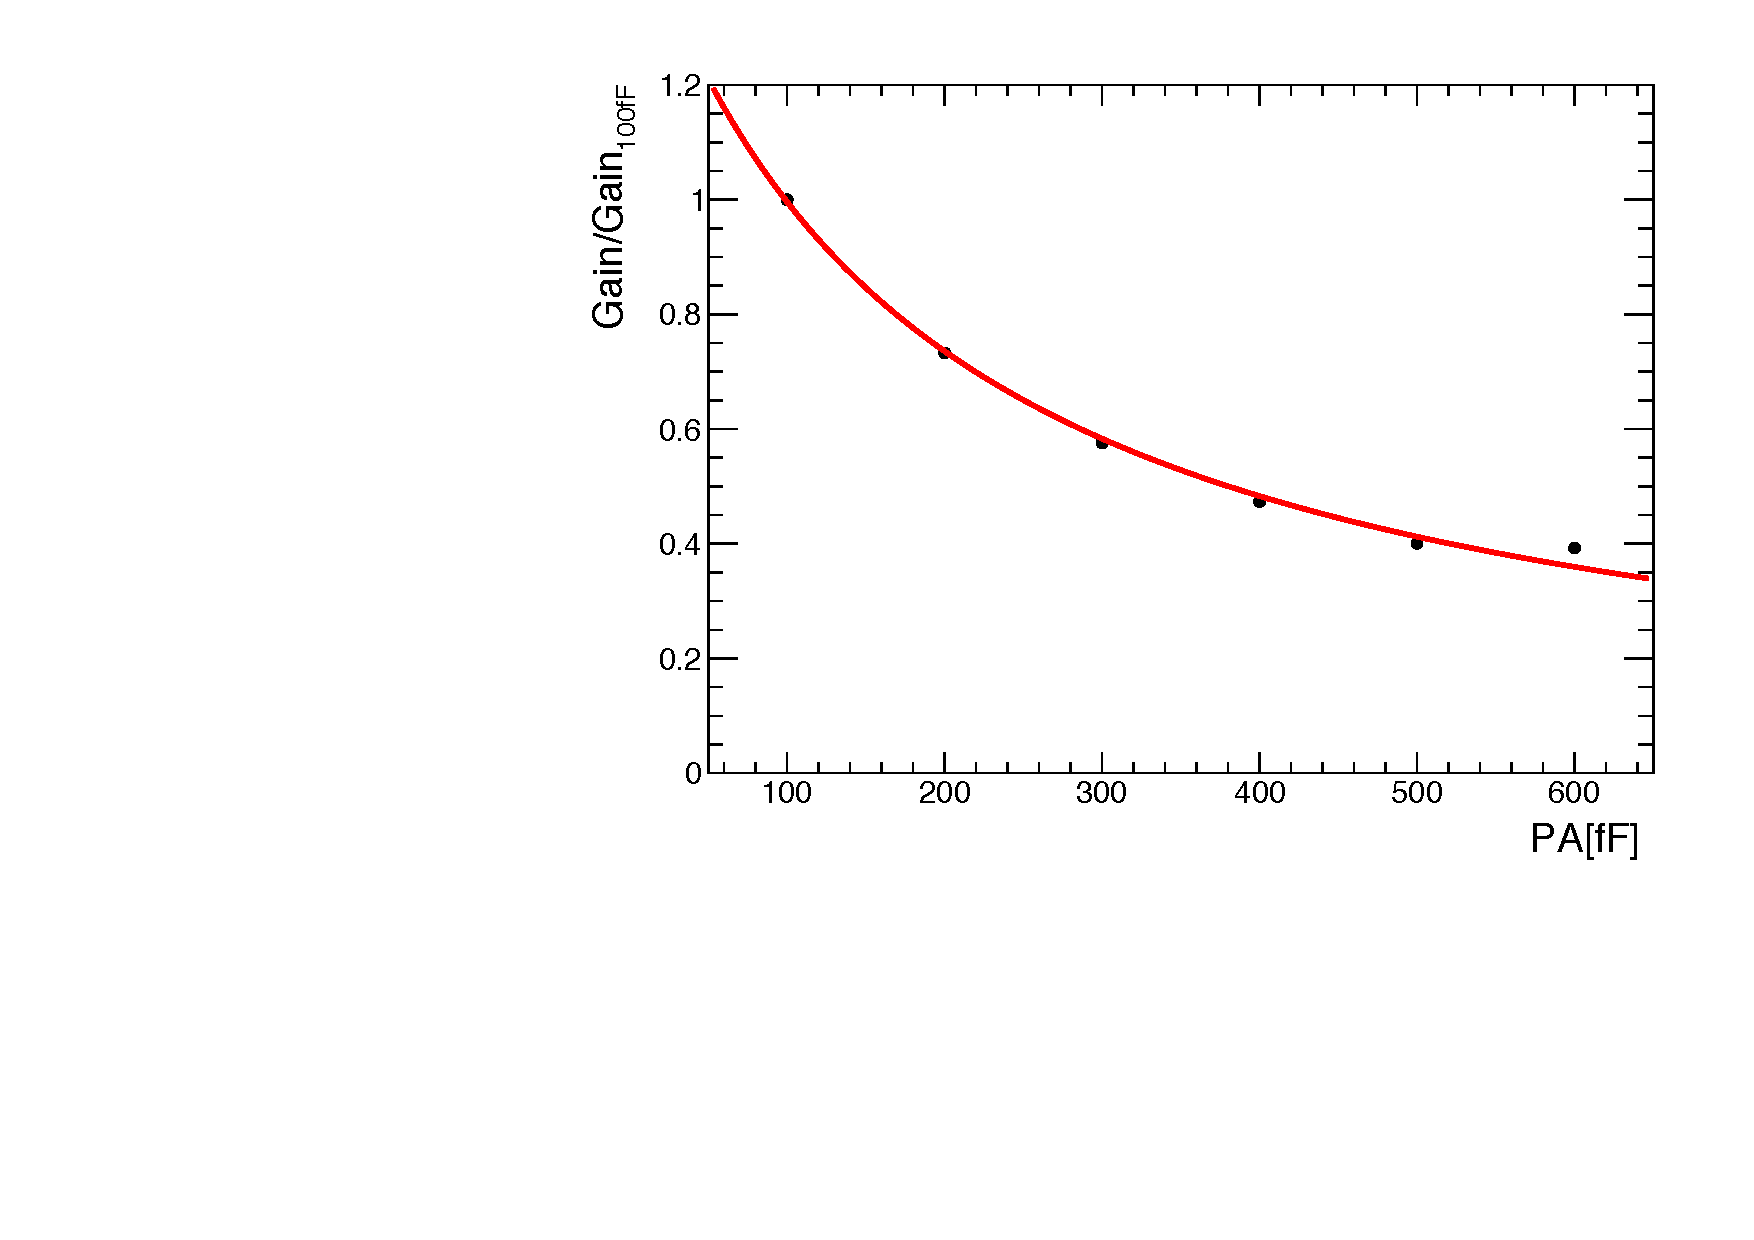
\includegraphics[width=1.\linewidth]{../Thesis_Plots/Commissioning/Plots/GainvsPA.pdf}
    \caption{} \label{fig:PA_curve}
  \end{subfigure}
  \hfill
  \begin{subfigure}[t]{0.49\textwidth}
    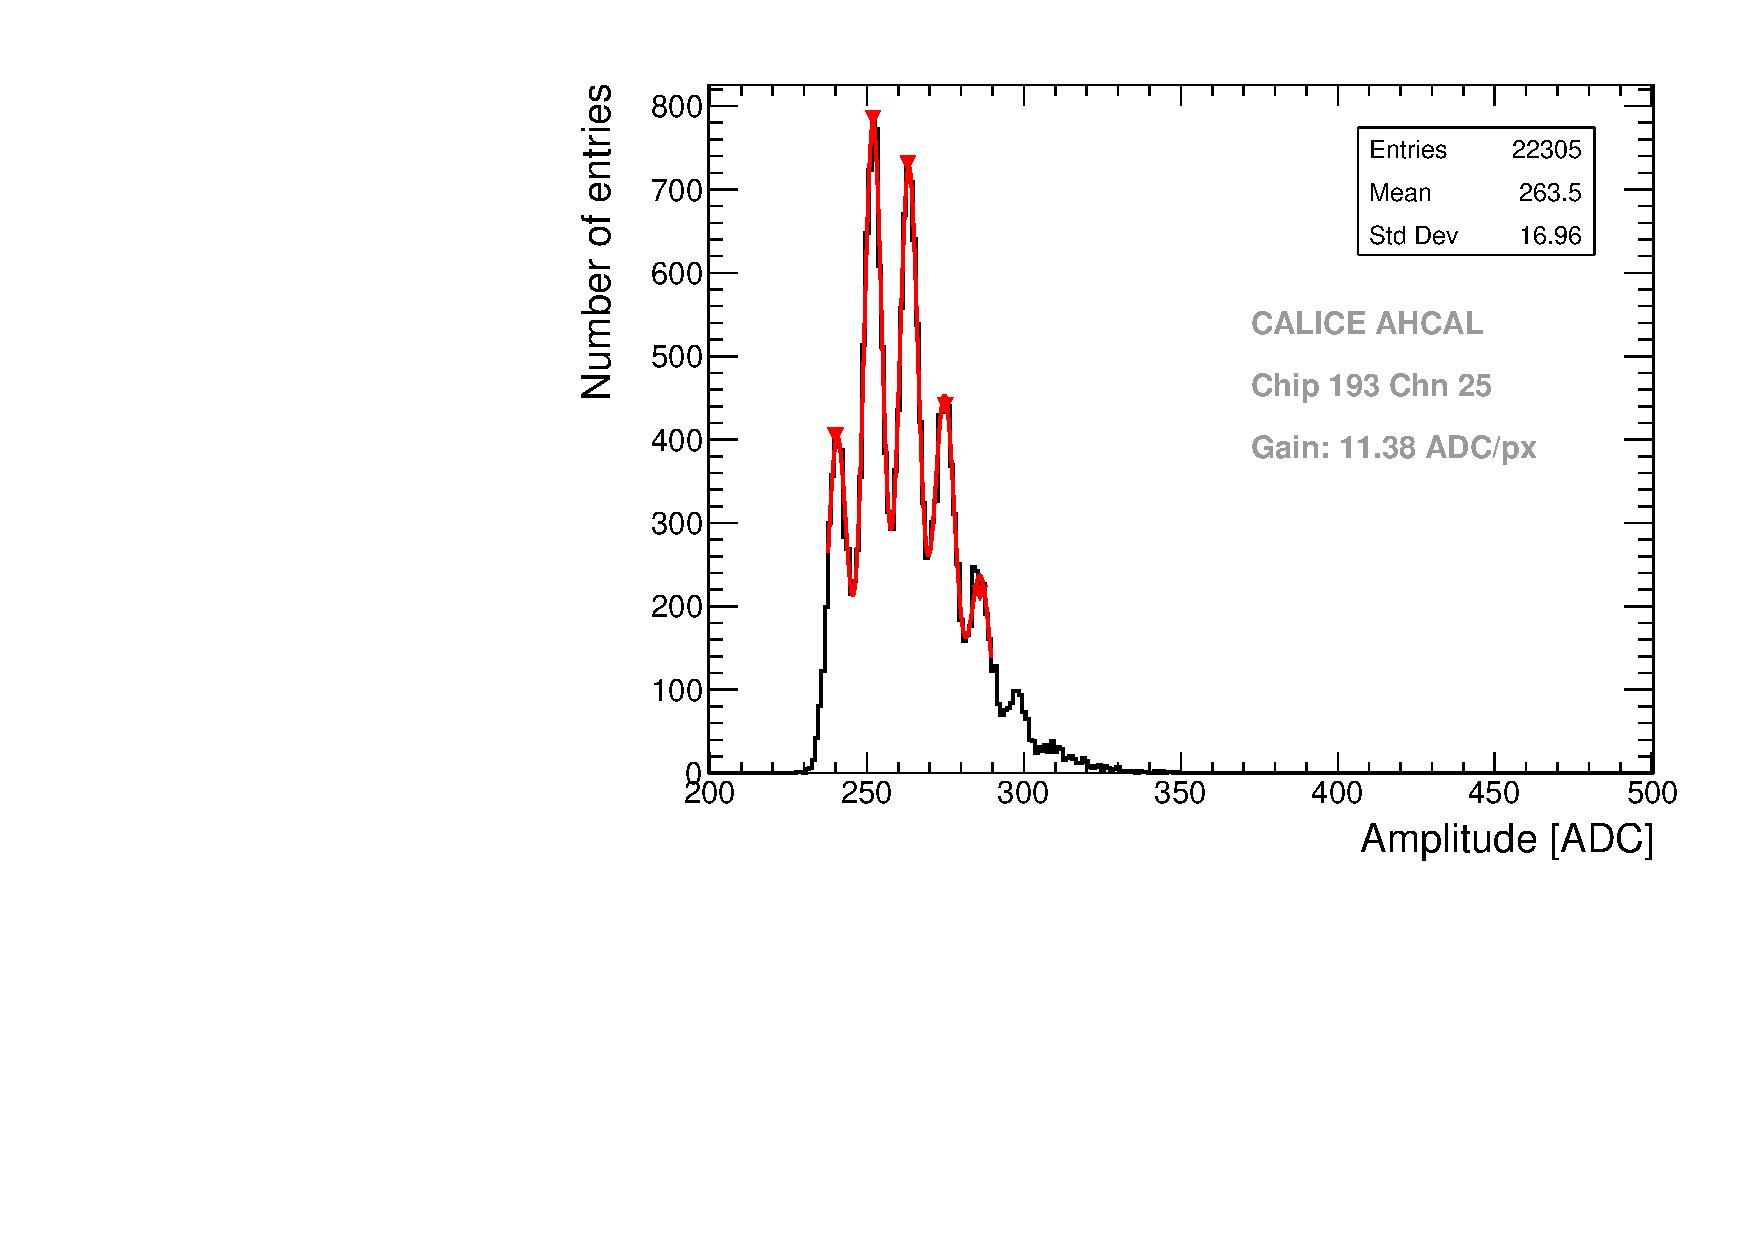
\includegraphics[width=1.\linewidth]{../Thesis_Plots/Commissioning/Plots/Gain675fF_MainzHBU4.pdf}
    \caption{} \label{fig:Gain675fF}
  \end{subfigure}
  \caption{\subref{fig:PA_curve}) Generic dependence of the gain as function of the pre-amplifier capacitance. obtained with the layer 4 used to determine the value of the pre-amplifier feedback capacitor to use. \subref{fig:Gain675fF}) Results of the gain fit for the same channel as shown above after adjustment of the pre-amplifier feedback capacitor from 100 fF to 675 fF.}
\end{figure}

\subsection{Threshold scan}

The SPIROC2B offers the possibility of setting a global trigger threshold (10-bit range) as well as an individual channel-wise threshold (4-bit range) in auto-trigger operation. The channel-wise threshold cannot be used currently as it induces a shift on the global threshold. The trigger threshold needs to be setup properly in order to avoid loss of information if set too high or being overwhelmed by noise events if set too low. The goal of this method is to get a good first estimate (to an order of 5-10\%) of the needed value for the trigger threshold in a quick and efficient way. Further adjustements in testbeam will depends on beam rates and noise conditions. A more complete description of the procedure can been found in \cite{Hartbrich:2016bbz} and \cite{LloydTrigger}.

\begin{figure}[htbp!]
  \centering
  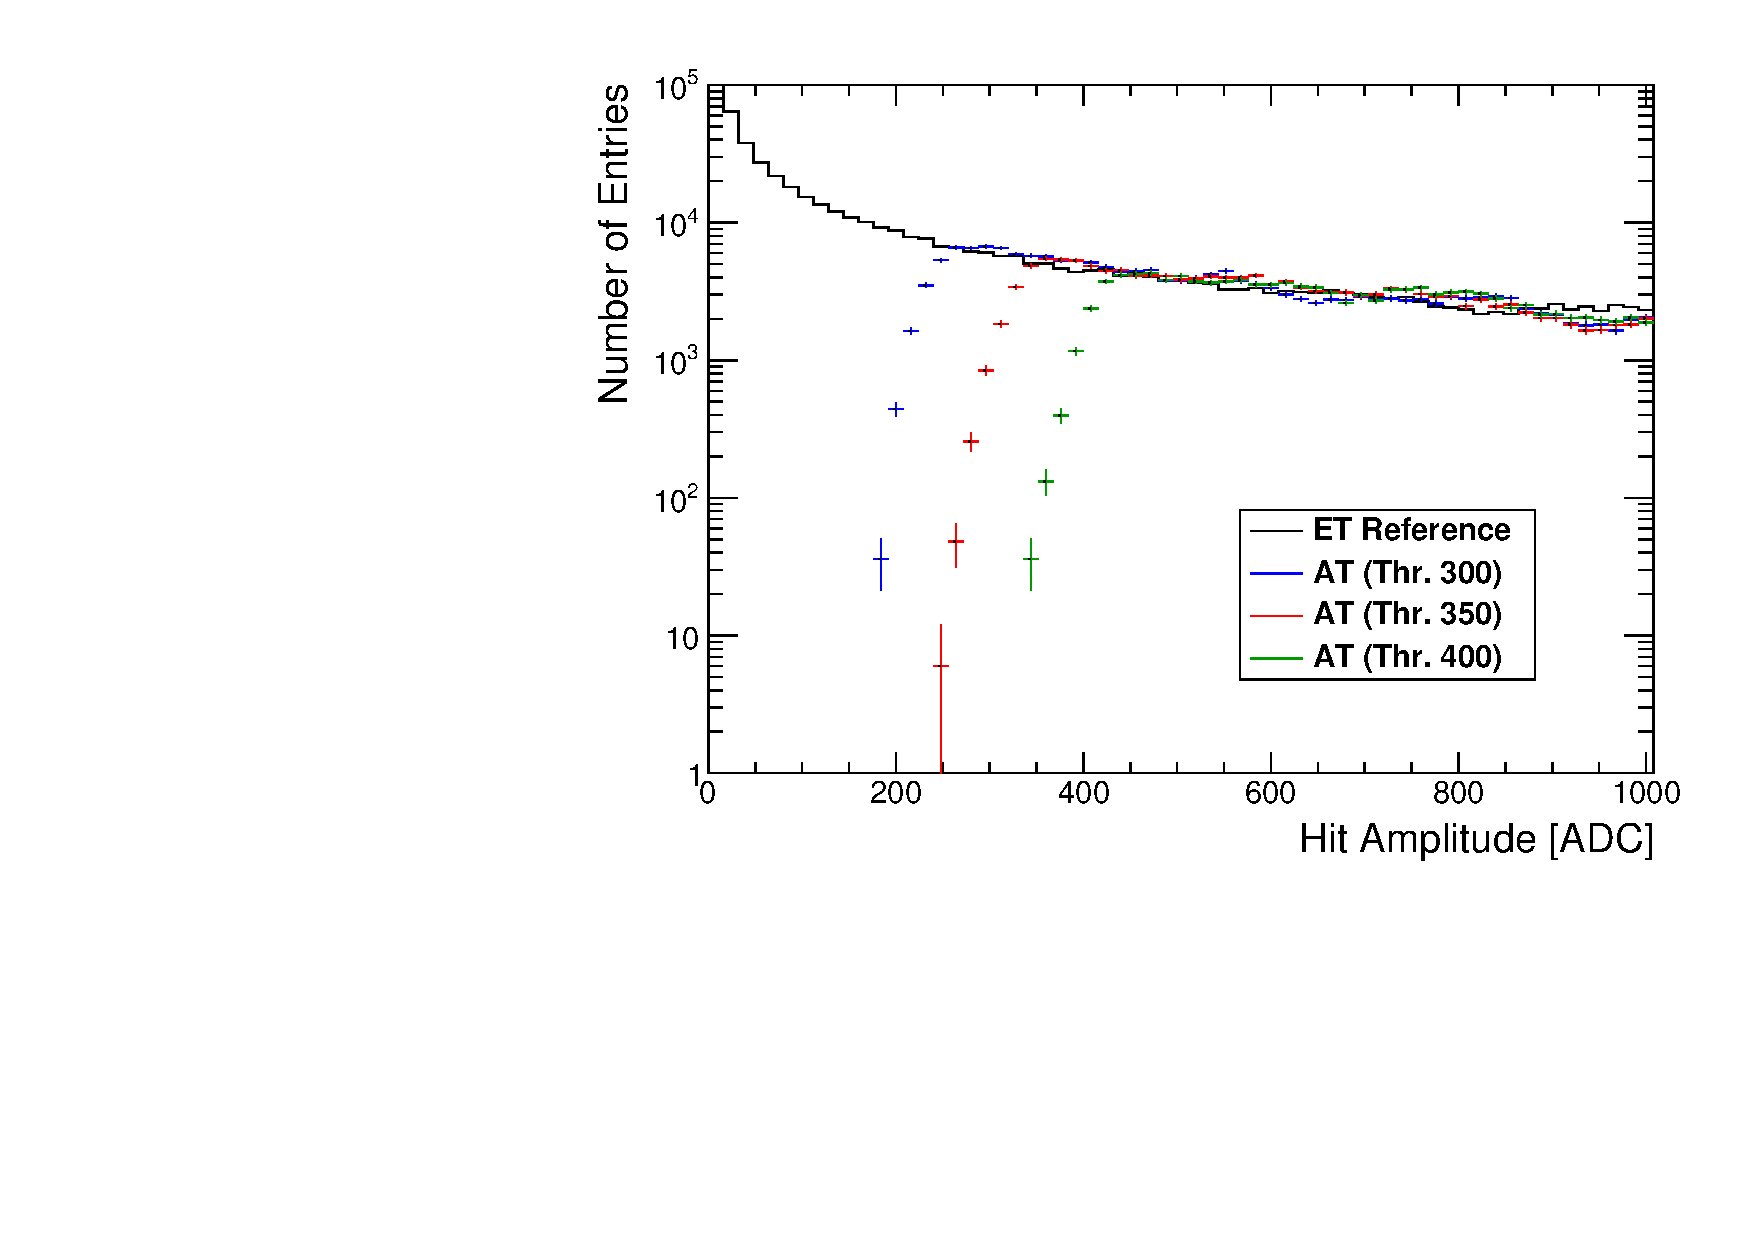
\includegraphics[width=0.6\linewidth]{../Thesis_Plots/Commissioning/Plots/SpectraADC_HBU2_12.pdf}
  \caption{ET reference spectrum and AT spectra of a single channel for different trigger threshold values of 300, 350 and 400. One can notice a clear dependence of the trigger position as a function of the threshold value.} \label{fig:ADCTriggerThreshold}
\end{figure}

The procedure utilizes the integrated LED calibration system to record a number of runs with increasing LED amplitude. For each LED amplitude, a run is taken in external trigger (ET) and then immediately followed by runs in auto-trigger (AT) with different trigger threshold configuration. This is done to ensure comparable LED amplitudes between the two runs as the LED amplitude is not stable over time. Next, the ADC of all ET runs are summed up into an histogram and the same is done for all AT runs for each trigger threshold value. An example of the spectra obtained for a single channel for three different thresholds is shown in figure \ref{fig:ADCTriggerThreshold}. It shows a clear dependence of the trigger threshold position as expected.

\begin{figure}[htbp!]
  \centering
  \begin{subfigure}[t]{0.49\textwidth}
    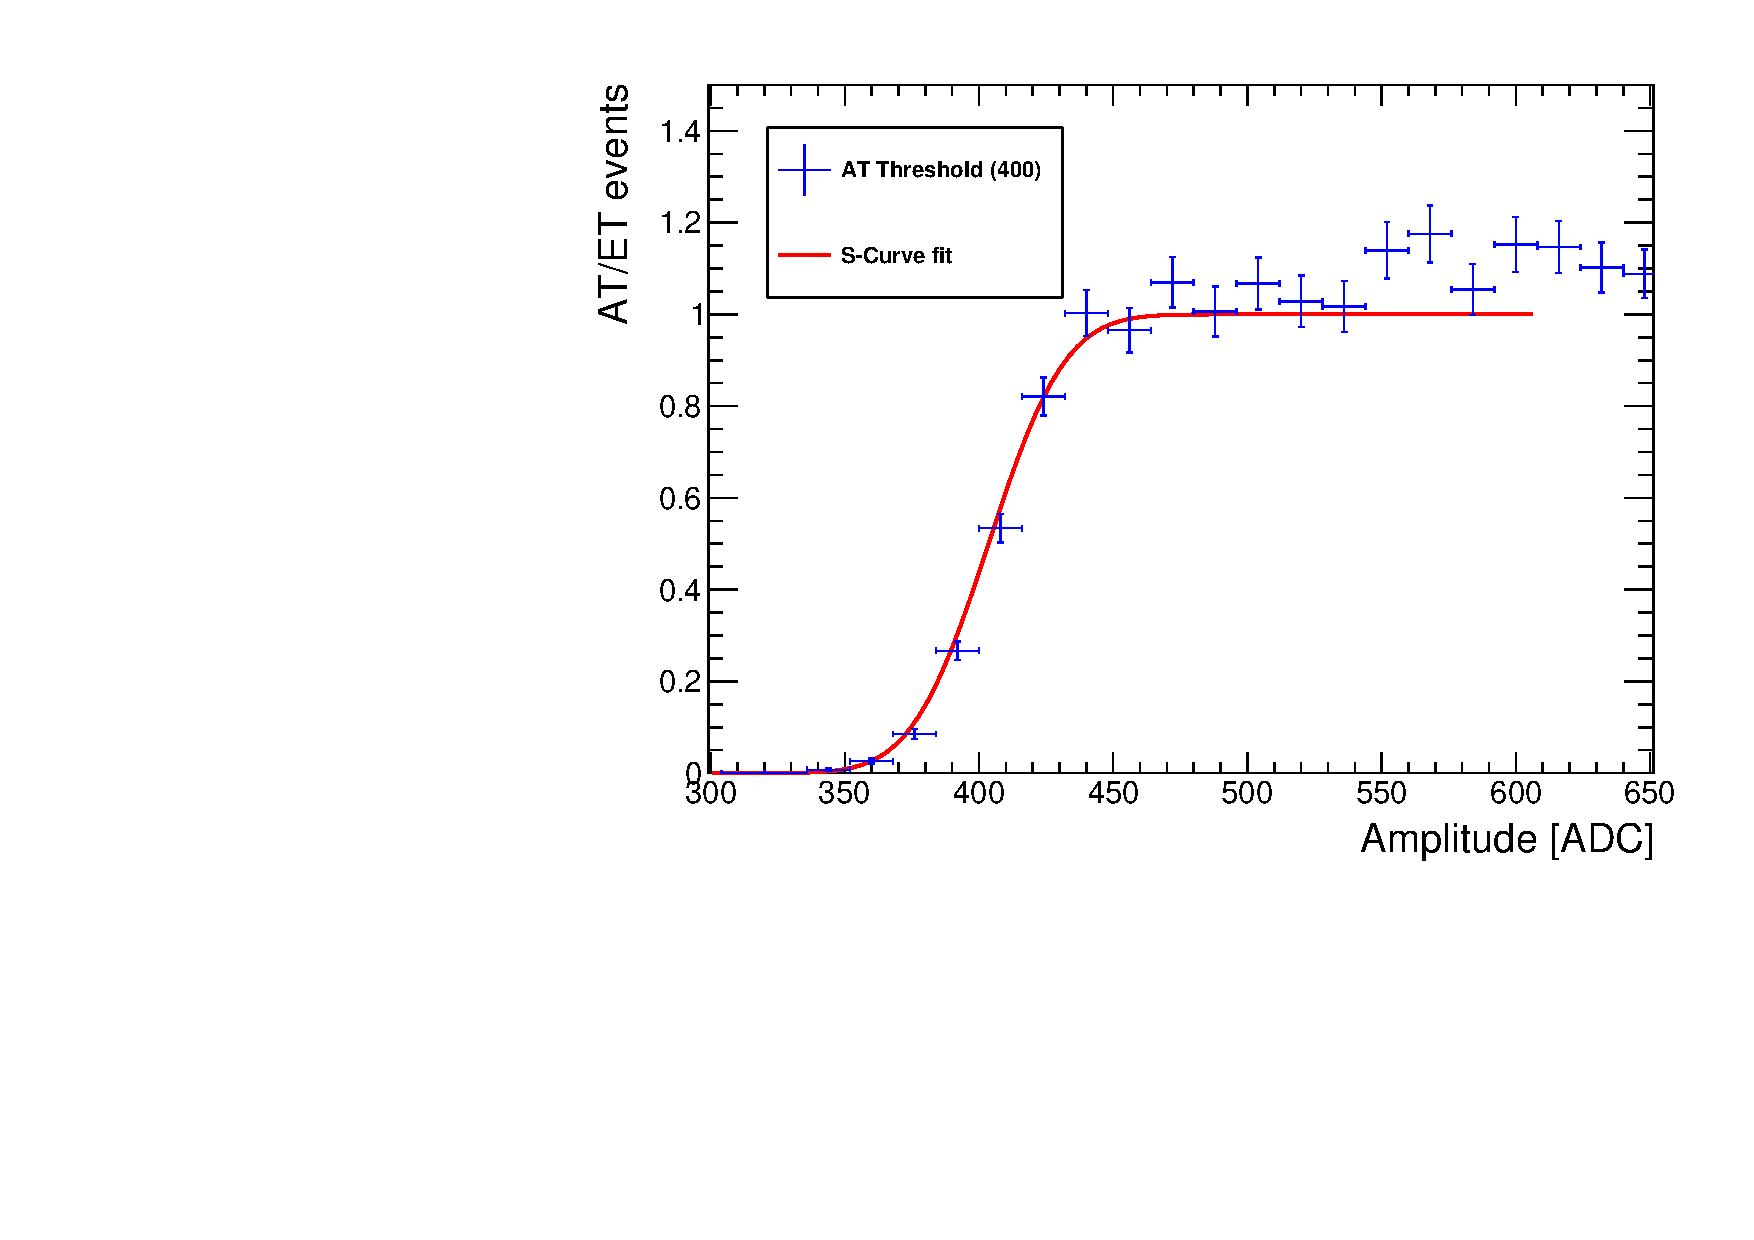
\includegraphics[width=1.\linewidth]{../Thesis_Plots/Commissioning/Plots/EfficiencyCurveFit_HBU2_12.pdf}
    \caption{} \label{fig:EffiCurve}
  \end{subfigure}
  \hfill
  \begin{subfigure}[t]{0.49\textwidth}
    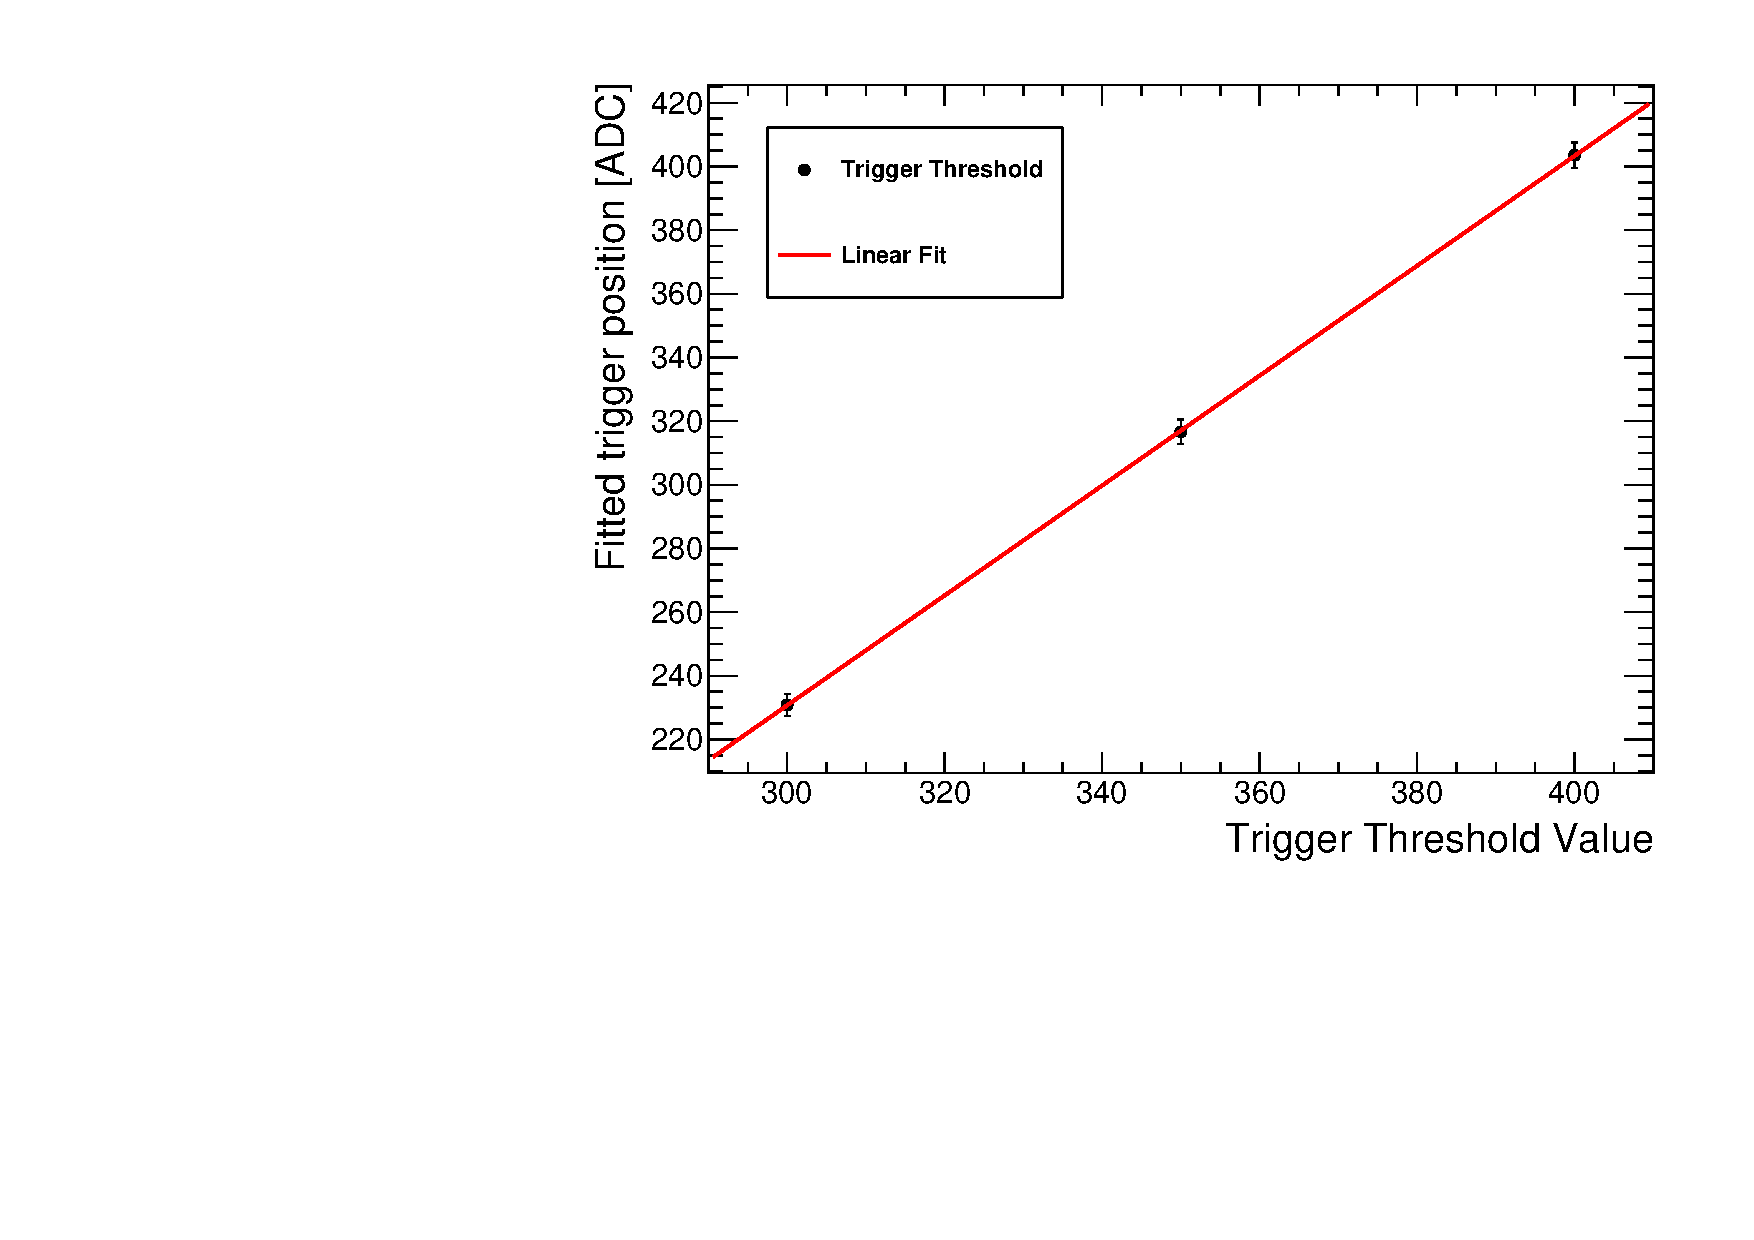
\includegraphics[width=1.\linewidth]{../Thesis_Plots/Commissioning/Plots/TriggerThresholdFit_HBU2_12.pdf}
    \caption{} \label{fig:TriggerFit}
  \end{subfigure}
  \caption{\subref{fig:EffiCurve}) Trigger efficiency S-Curve fit for a typical channel at a trigger threshold of 400. $\mu$ = 403.542 $\pm$ 4.04538. \subref{fig:TriggerFit}) Extracted trigger threshold positions as a function of the trigger threshold value. One can observe a linear behavior.}
\end{figure}

By dividing the ET reference spectrum with the AT spectrum, an efficiency curve is obtained for each trigger threshold configuration. This efficiency curve can be fitted with an \textit{error function} $erf(x)$ of parameters $\sigma$ and $\mu$ for the width and position. An example of the fit for a single channel and trigger threshold configuration is shown in figure \ref{fig:EffiCurve}. The efficiency is normalized to 1 due to the measurement method. The statistical uncertainty on the trigger position is around 1\% which is well below the needed accuracy. The fit is repeated for each trigger threshold configuration and the dependence of the trigger position as function of the threshold parameter can be drawn (see figure \ref{fig:TriggerFit}). The dependence of the trigger position on the threshold parameter is linear as expected.

This method was performed on 14 fully equipped HBUs \cite{LloydTrigger}. The dependence of the trigger position on the threshold parameter was obtained for most channels. The trigger threshold for each channel is then determined at 0.5 MIP using the linear dependence, for this, an assumption of the MIP value for each channel is made based on the target light yield and gain as no MIP measurement was available at the time. The trigger threshold per chip to use is the minimum trigger threshold extracted for all the 36 channels.

\section{Noise Measurement in the AHCAL}

Noise measurement is needed and is a measurement that gives additional information on the trigger threshold. As explained above, the setting of the trigger threshold is very crucial. If the threshold is set too low, a noisy channel could overflow the whole detector thus reducing the readout efficiency. Noise measurements has already been done in the past for 4 HBU boards in 2012 \cite{Hermberg:2015gaa}. This method is a proof-of-concept that seems to fulfill the requirement of characterizing the noise as a function of the threshold position for all the channels or a chip at once. The needed accuracy is also here not so crucial in order to keep the threshold in the acceptable range of 0.5 MIP. This method enables us to have an idea of the noise level at a certain trigger threshold and especially to understand the evolution of noise as a function of the trigger threshold. This measurement method utilizes the fact that SiPM noise should follow a Poisson distribution. Moreover, to eliminate the dependence of the SiPM noise as a function of the temperature, the measurement is performed in a climate chamber at a temperature of 25 degrees Celsius.

Each measurement is taken in auto-trigger mode for different time windows ($T$), from 1 ms to 30 ms, for different values of the trigger threshold from 200 to 250. Each measurement is done 200 times (readout cycles). For each cycle, the number of filled memory cells is put into a histogram per chip. It is checked that the bin 15 of the histogram, i.e corresponding to the memory cell 16, is not filled otherwise the chip would be automatically read out. This is done to ensure that the measurement is stopped at exactly the end of the time window and not before. In a next step, each histogram is fitted with a Poisson distribution. A typical example of a chip can be seen in figure \ref{fig:MemPoison}. The most probable value (MPV) $\lambda_{mem}$ of the Poisson distribution gives the most probable number of memory cells filled per chip for a specific trigger threshold value and time window $T$.

This can then be converted into a noise rate as $\textit{Noise Rate} = \frac{\lambda_{mem}}{T}$ and filled into an histogram per chip for each trigger threshold value. The mean value of the noise rate per chip for each trigger threshold value is used to plot the noise rate as a function of the trigger threshold value for each chip. The figure \ref{fig:DCRThr} shows the results obtained for a typical board.

\begin{figure}[htbp!]
  \centering
  \begin{subfigure}[t]{0.49\textwidth}
    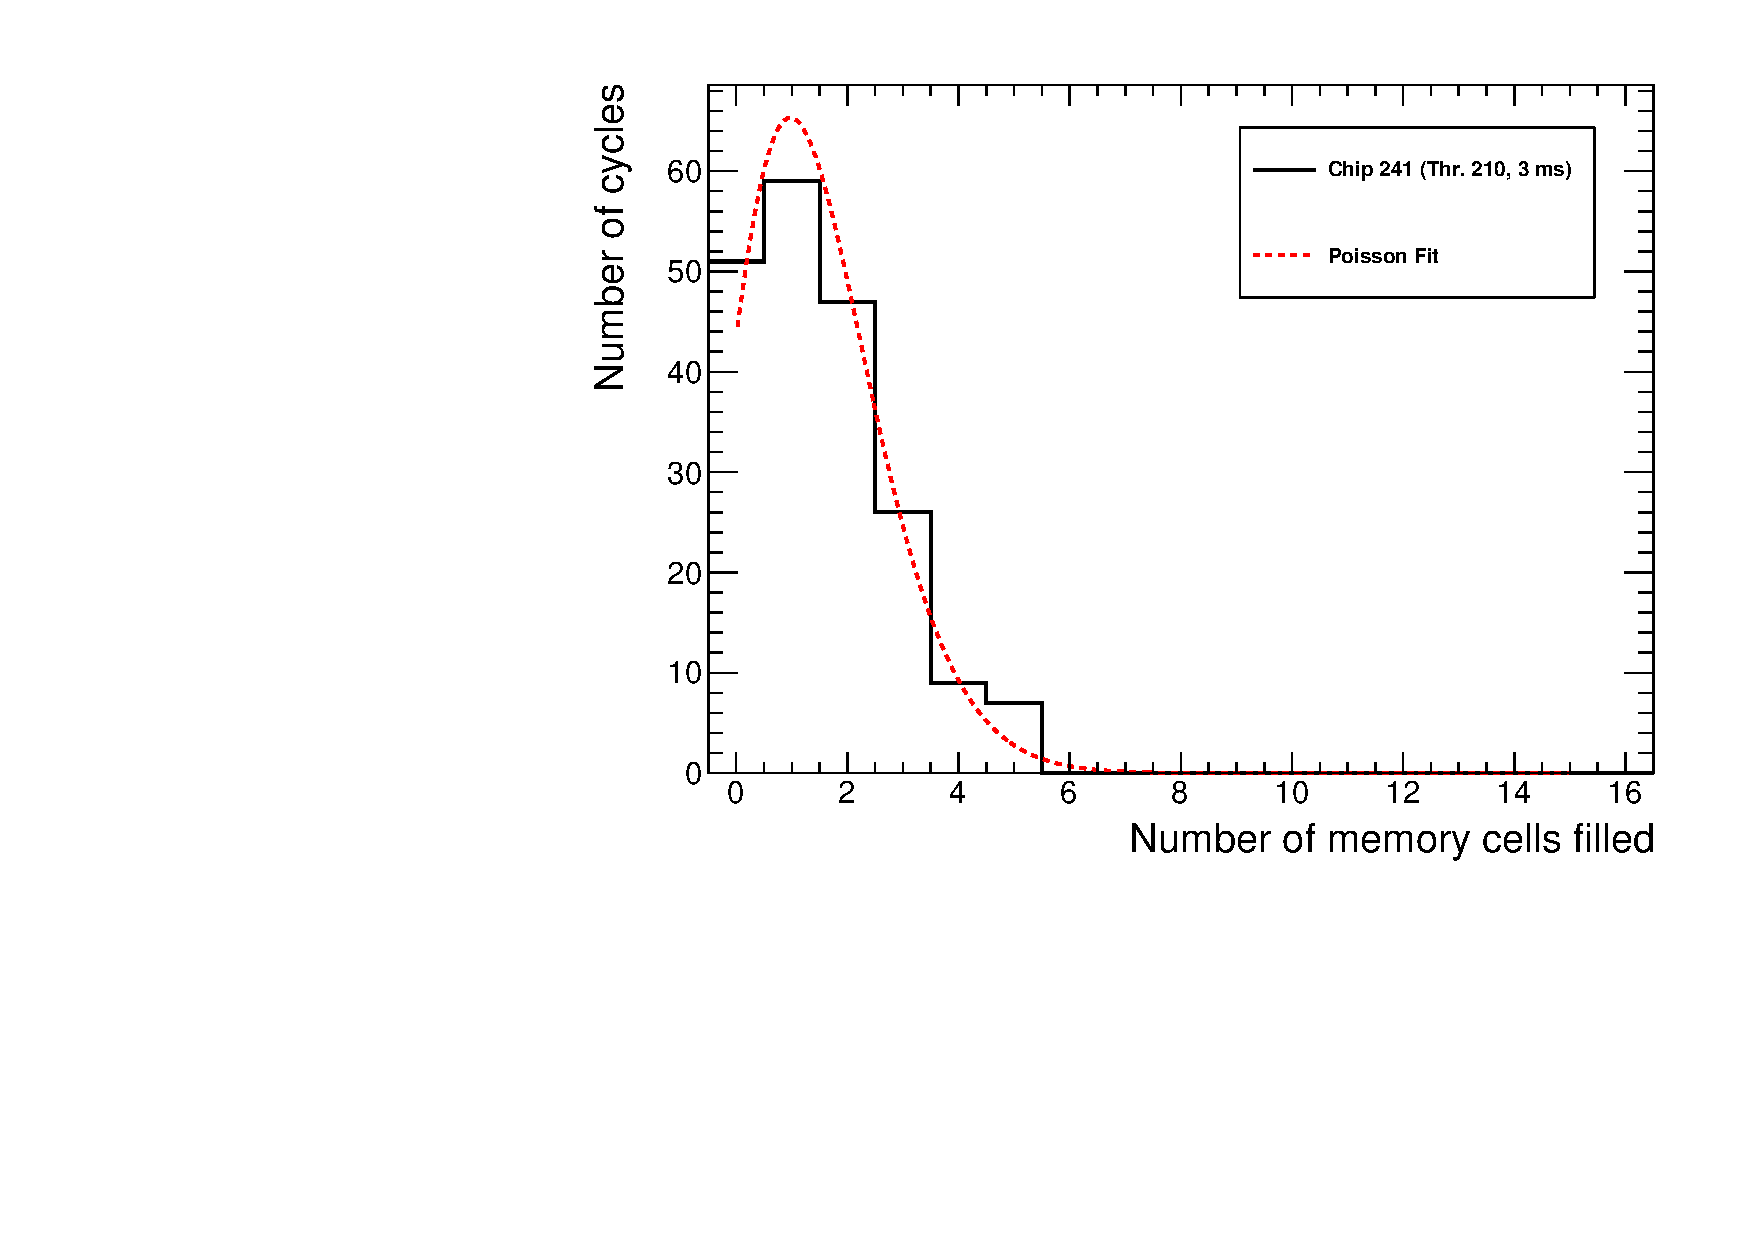
\includegraphics[width=1.\linewidth]{../Thesis_Plots/Commissioning/Plots/NumberMemFilled_Poisson.pdf}
    \caption{} \label{fig:MemPoison}
  \end{subfigure}
  \hfill
  \begin{subfigure}[t]{0.49\textwidth}
    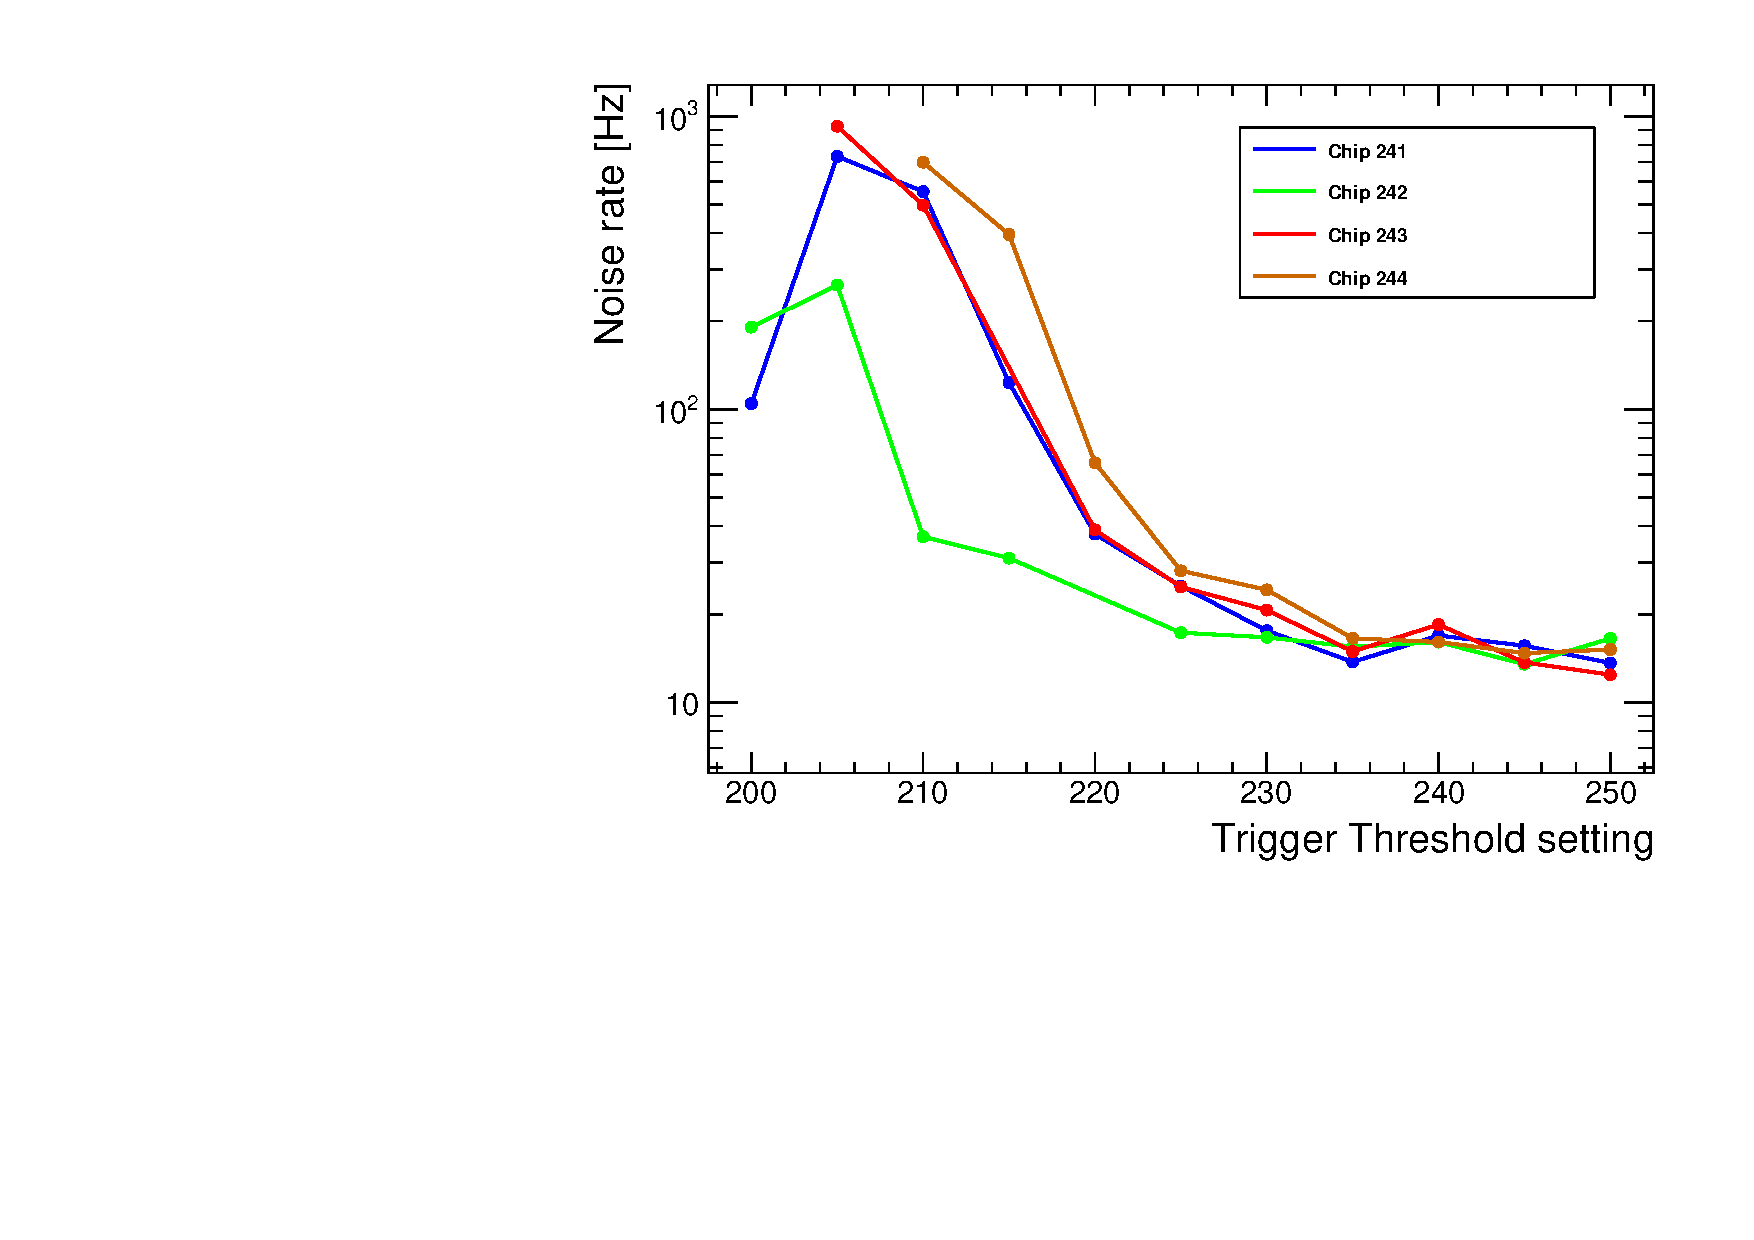
\includegraphics[width=1.\linewidth]{../Thesis_Plots/Commissioning/Plots/NoiseMeasurement_SM1.pdf}
    \caption{} \label{fig:DCRThr}
  \end{subfigure}
  \caption{\subref{fig:MemPoison}) Observed histogram of the number of memory cells filled per cycle for a typical chip with a trigger threshold of 210 and a time window $T$ of 3 ms. $\lambda_{mem}$ = 1.5 $\pm$ 0.1.\subref{fig:DCRThr}) Extracted noise rate as a function of the trigger threshold setting for a full board.}
\end{figure}

The figure \ref{fig:DCRThr} shows that noise decreases fast with increasing threshold until a plateau is reached. This plateau is the ideal area to set the threshold as noise is quite constant. In this figure, a threshold between 230 and 240 seems appropriate. As this method is complementary to the threshold scan, the region can be compared to where is the threshold put in terms of MIP value. For this board, a threshold of 230-240 corresponds to about a threshold 0.2-0.25 MIP which is well below 0.5 MIP and thus safe.

This method is very complementary to the threshold scan and can be used to set a relatively safe trigger threshold for all chips. It does not rely on a very precise measurement and has been shown to work well for all chips. Moreover, this method requires only minimal additional time to the commissioning procedure. A full understanding of the position of the trigger threshold relative to 0.5 MIP would greatly improve the data taking efficiency of future AHCAL engineering prototypes.

\begin{center}
  \rule{0.5\textwidth}{.4pt}
\end{center}

This chapter presents the ASIC testing and commissioning procedure for the AHCAL technological prototype performed during the summer of 2014. First, around 60 chips have been tested manually with a yield of 84\% to be equipped on new HBU boards. The testing procedure aims at reducing the number of dead channels by testing crucial features of the chip. The time to test each ASIC is around 10 minutes.

The commissioning of AHCAL boards is divided in several procedures described in this chapter. In total, three EBU and 24 HBU boards have been commissioned in the year 2014-2015. The total time for the procedure varies between one hour, for the new generation boards, to 7-8 hours depending on the LED amplitude range needed. In the future, the commissioning procedure can be improved by the calibration of the HBU in a cosmic-stand providing a reliable cross-check along the production before a full calibration in testbeam.

After the commissioning, a full assembled AHCAL prototype was placed in various beams at the CERN SPS facilities during the summer of 2015. In the following chapters, an analysis of the collected testbeam data focused on the time development of hadronic showers is presented.
